% Template for PLoS
% Version 3.5 March 2018
%
% % % % % % % % % % % % % % % % % % % % % %
%
% -- IMPORTANT NOTE
%
% This template contains comments intended 
% to minimize problems and delays during our production 
% process. Please follow the template instructions
% whenever possible.
%
% % % % % % % % % % % % % % % % % % % % % % % 
%
% Once your paper is accepted for publication, 
% PLEASE REMOVE ALL TRACKED CHANGES in this file 
% and leave only the final text of your manuscript. 
% PLOS recommends the use of latexdiff to track changes during review, as this will help to maintain a clean tex file.
% Visit https://www.ctan.org/pkg/latexdiff?lang=en for info or contact us at latex@plos.org.
%
%
% There are no restrictions on package use within the LaTeX files except that 
% no packages listed in the template may be deleted.
%
% Please do not include colors or graphics in the text.
%
% The manuscript LaTeX source should be contained within a single file (do not use \input, \externaldocument, or similar commands).
%
% % % % % % % % % % % % % % % % % % % % % % %
%
% -- FIGURES AND TABLES
%
% Please include tables/figure captions directly after the paragraph where they are first cited in the text.
%
% DO NOT INCLUDE GRAPHICS IN YOUR MANUSCRIPT
% - Figures should be uploaded separately from your manuscript file. 
% - Figures generated using LaTeX should be extracted and removed from the PDF before submission. 
% - Figures containing multiple panels/subfigures must be combined into one image file before submission.
% For figure citations, please use "Fig" instead of "Figure".
% See http://journals.plos.org/plosone/s/figures for PLOS figure guidelines.
%
% Tables should be cell-based and may not contain:
% - spacing/line breaks within cells to alter layout or alignment
% - do not nest tabular environments (no tabular environments within tabular environments)
% - no graphics or colored text (cell background color/shading OK)
% See http://journals.plos.org/plosone/s/tables for table guidelines.
%
% For tables that exceed the width of the text column, use the adjustwidth environment as illustrated in the example table in text below.
%
% % % % % % % % % % % % % % % % % % % % % % % %
%
% -- EQUATIONS, MATH SYMBOLS, SUBSCRIPTS, AND SUPERSCRIPTS
%
% IMPORTANT
% Below are a few tips to help format your equations and other special characters according to our specifications. For more tips to help reduce the possibility of formatting errors during conversion, please see our LaTeX guidelines at http://journals.plos.org/plosone/s/latex
%
% For inline equations, please be sure to include all portions of an equation in the math environment.  For example, x$^2$ is incorrect; this should be formatted as $x^2$ (or $\mathrm{x}^2$ if the romanized font is desired).
%
% Do not include text that is not math in the math environment. For example, CO2 should be written as CO\textsubscript{2} instead of CO$_2$.
%
% Please add line breaks to long display equations when possible in order to fit size of the column. 
%
% For inline equations, please do not include punctuation (commas, etc) within the math environment unless this is part of the equation.
%
% When adding superscript or subscripts outside of brackets/braces, please group using {}.  For example, change "[U(D,E,\gamma)]^2" to "{[U(D,E,\gamma)]}^2". 
%
% Do not use \cal for caligraphic font.  Instead, use \mathcal{}
%
% % % % % % % % % % % % % % % % % % % % % % % % 
%
% Please contact latex@plos.org with any questions.
%
% % % % % % % % % % % % % % % % % % % % % % % %

\documentclass[10pt,letterpaper]{article}
\usepackage[top=0.85in,left=2.75in,footskip=0.75in]{geometry}

% amsmath and amssymb packages, useful for mathematical formulas and symbols
\usepackage{amsmath,amssymb}

% Use adjustwidth environment to exceed column width (see example table in text)
\usepackage{changepage}

% Use Unicode characters when possible
\usepackage[utf8x]{inputenc}

% textcomp package and marvosym package for additional characters
\usepackage{textcomp,marvosym}

% cite package, to clean up citations in the main text. Do not remove.
\usepackage{cite}

% Use nameref to cite supporting information files (see Supporting Information section for more info)
\usepackage{nameref,hyperref}

% line numbers
\usepackage[right]{lineno}

% ligatures disabled
\usepackage{microtype}
\DisableLigatures[f]{encoding = *, family = * }

% color can be used to apply background shading to table cells only
\usepackage[table]{xcolor}

% array package and thick rules for tables
\usepackage{array}

% create "+" rule type for thick vertical lines
\newcolumntype{+}{!{\vrule width 2pt}}

% create \thickcline for thick horizontal lines of variable length
\newlength\savedwidth
\newcommand\thickcline[1]{%
  \noalign{\global\savedwidth\arrayrulewidth\global\arrayrulewidth 2pt}%
  \cline{#1}%
  \noalign{\vskip\arrayrulewidth}%
  \noalign{\global\arrayrulewidth\savedwidth}%
}

% \thickhline command for thick horizontal lines that span the table
\newcommand\thickhline{\noalign{\global\savedwidth\arrayrulewidth\global\arrayrulewidth 2pt}%
\hline
\noalign{\global\arrayrulewidth\savedwidth}}


% Remove comment for double spacing
%\usepackage{setspace} 
%\doublespacing

% Text layout
\raggedright
\setlength{\parindent}{0.5cm}
\textwidth 5.25in 
\textheight 8.75in

% Bold the 'Figure #' in the caption and separate it from the title/caption with a period
% Captions will be left justified
\usepackage[aboveskip=1pt,labelfont=bf,labelsep=period,justification=raggedright,singlelinecheck=off]{caption}
\renewcommand{\figurename}{Fig}

% Use the PLoS provided BiBTeX style
\bibliographystyle{plos2015}

% Remove brackets from numbering in List of References
\makeatletter
\renewcommand{\@biblabel}[1]{\quad#1.}
\makeatother



% Header and Footer with logo
\usepackage{lastpage,fancyhdr,graphicx}
\usepackage{epstopdf}
%\pagestyle{myheadings}
\pagestyle{fancy}
\fancyhf{}
%\setlength{\headheight}{27.023pt}
%\lhead{\includegraphics[width=2.0in]{PLOS-submission.eps}}
\rfoot{\thepage/\pageref{LastPage}}
\renewcommand{\headrulewidth}{0pt}
\renewcommand{\footrule}{\hrule height 2pt \vspace{2mm}}
\fancyheadoffset[L]{2.25in}
\fancyfootoffset[L]{2.25in}
\lfoot{\today}

%% Include all macros below

\newcommand{\lorem}{{\bf LOREM}}
\newcommand{\ipsum}{{\bf IPSUM}}

%% my packages and configs
\usepackage{longtable}
\usepackage{booktabs}
\usepackage{url}
\def\UrlBreaks{\do\/\do-}

%% END MACROS SECTION


\begin{document}
\vspace*{0.2in}

% Title must be 250 characters or less.
\begin{flushleft}
{\Large
\textbf\newline{Causal graph analysis of COVID-19 observational data in German districts reveals effects of determining factors on reported case numbers} % Please use "sentence case" for title and headings (capitalize only the first word in a title (or heading), the first word in a subtitle (or subheading), and any proper nouns).
}
\newline
% Insert author names, affiliations and corresponding author email (do not include titles, positions, or degrees).
\\
Edgar Steiger\textsuperscript{1*},
Tobias Mussgnug\textsuperscript{1},
Lars Eric Kroll\textsuperscript{1}%,
%Name4 Surname\textsuperscript{2},
%Name5 Surname\textsuperscript{2\ddag},
%Name6 Surname\textsuperscript{2\ddag},
%Name7 Surname\textsuperscript{1,2,3*},
%with the Lorem Ipsum Consortium\textsuperscript{\textpilcrow}
\\
\bigskip
\textbf{1} Central Research Institute of Ambulatory Health Care in Germany (Zi),
Salzufer 8, D-10587 Berlin, Germany
\\
%\textbf{2} Affiliation Dept/Program/Center, Institution Name, City, State, Country
%\\
%\textbf{3} Affiliation Dept/Program/Center, Institution Name, City, State, Country
%\\
\bigskip

% Insert additional author notes using the symbols described below. Insert symbol callouts after author names as necessary.
% 
% Remove or comment out the author notes below if they aren't used.
%
% Primary Equal Contribution Note
%\Yinyang These authors contributed equally to this work.

% Additional Equal Contribution Note
% Also use this double-dagger symbol for special authorship notes, such as senior authorship.
%\ddag These authors also contributed equally to this work.

% Current address notes
%\textcurrency Current Address: Dept/Program/Center, Institution Name, City, State, Country % change symbol to "\textcurrency a" if more than one current address note
% \textcurrency b Insert second current address 
% \textcurrency c Insert third current address

% Deceased author note
%\dag Deceased

% Group/Consortium Author Note
%\textpilcrow Membership list can be found in the Acknowledgments section.

% Use the asterisk to denote corresponding authorship and provide email address in note below.
* esteiger@zi.de

\end{flushleft}
% Please keep the abstract below 300 words
\section*{Abstract}
Several determinants are suspected to be causal drivers for new cases of COVID-19 infection. Correcting for possible confounders, we estimated the effects of the most prominent determining factors on reported case numbers. To this end, we used a directed acyclic graph (DAG) as a graphical representation of the hypothesized causal effects of the determinants on new reported cases of COVID-19. Based on this, we computed valid adjustment sets of the possible confounding factors. We collected data for Germany from publicly available sources (e.g.~Robert Koch Institute, Germany's National Meteorological Service, Google) for 401 German districts over the period of 15 February to 8 July 2020, and estimated total causal effects based on our DAG analysis by negative binomial regression. Our analysis revealed favorable effects of increasing temperature, increased public mobility for essential shopping (grocery and pharmacy) or within residential areas, and awareness measured by COVID-19 burden, all of them reducing the outcome of newly reported COVID-19 cases. Conversely, we saw adverse effects leading to an increase in new COVID-19 cases for public mobility in retail and recreational areas or workplaces, awareness measured by searches for ``corona'' in Google, higher rainfall, and some socio-demographic factors. Non-pharmaceutical interventions were found to be effective in reducing case numbers. This comprehensive causal graph analysis of a variety of determinants affecting COVID-19 progression gives strong evidence for the driving forces of mobility, public awareness, and temperature, whose implications need to be taken into account for future decisions regarding pandemic management.

% Please keep the Author Summary between 150 and 200 words
% Use first person. PLOS ONE authors please skip this step. 
% Author Summary not valid for PLOS ONE submissions.   
%\section*{Author summary}
%Lorem ipsum dolor sit amet, consectetur adipiscing elit. Curabitur eget porta erat. Morbi consectetur est vel gravida pretium. Suspendisse ut dui eu ante cursus gravida non sed sem. Nullam sapien tellus, commodo id velit id, eleifend volutpat quam. Phasellus mauris velit, dapibus finibus elementum vel, pulvinar non tellus. Nunc pellentesque pretium diam, quis maximus dolor faucibus id. Nunc convallis sodales ante, ut ullamcorper est egestas vitae. Nam sit amet enim ultrices, ultrices elit pulvinar, volutpat risus.

\linenumbers

% Use "Eq" instead of "Equation" for equation citations.
\section*{Introduction}\label{introduction}
As the COVID-19 pandemic progresses, research on mechanisms behind the transmission of SARS-CoV-2 shows conflicting evidence \cite{who2020report, Chinazzi395, guan2020clinical}. While effects of mobility have been extensively discussed, less is known on other factors such as changing awareness in the population
\cite{higgins_correlations_2020, li_retrospective_2020, yuan_trends_2020}
or the effects of temperature
\cite{bannister-tyrrell_preliminary_2020, demongeot_temperature_2020, liu_impact_2020}. A limiting factor in many studies is the lack of a causal approach to
assess the causal contributions of various factors
\cite{Greenland1999}. This can lead to distorted estimates of the
causal factors with observational data
\cite{Greenland1999, schipf_directed_2011, textor_robust_2017}.

With COVID-19, we find ourselves in a situation in which information on
the causal contribution of various influencing factors in the population
is urgently needed to inform politicians and health authorities. On the
other hand, trials cannot be carried out for obvious ethical and legal
reasons. Therefore, when assessing the effects of determinants of
SARS-CoV-2 spread, special attention must be paid to strategies for the
selection of confounding factors.

Another problem with assessing the effects of various determinants of
SARS-CoV-2 spread is the heterogeneity of the countries and regions
examined for example in the Johns Hopkins University (JHU) COVID-19
database \cite{jhucovid19db2020}. The comparison of time series of case
numbers from different countries and observational periods can be
strongly distorted by different factors like testing capacities and
regional variations.

Our objective is to provide valid estimates of the effects of the main drivers of the pandemic with a causal graph approach. We conducted a scoping review of the available studies regarding signaling pathways and determinants of the spread of SARS-CoV-2 infections and the reported new COVID-19 cases. Then we integrated the current findings into a directed acyclic graph for the progress of the pandemic at the regional level. Using the resulting model and the do-calculus we found identifiable effects without blocked causal paths whose effects can be analyzed with observational data \cite{Pearl_2014}. We used regional time series data of all German districts (\(401\)) from various publicly available sources to analyze these questions on a regional level. Germany is a good choice in this regard, because it has ample data on contributing factors on the regional level and has had high testing and treatment capacities from early on in the pandemic.

\section*{Causal Model}\label{causal-model}

We used a directed acyclic graph (DAG)
\cite{schipf_directed_2011, textor_robust_2017} as a tool to analyze
the causal relationships between several exposures and SARS-CoV-2
spread. To get an overview on published associations, a scoping review
was conducted from 20th to 22nd of May 2020 within Pubmed and Google
scholar. Restrictions were applied to English and German language and
the publication date in the last one year. The following search terms
were applied to abstracts and title in Pubmed (``COVID-19'' OR
``COVID19'' OR ``Corona'' OR ``Coronavirus'' OR ``SARS-CoV-2'') and
connected separately in each case with the exposure variables
(``mobility'', ``public awareness'', ``awareness'', ``google
trends'',``ambient temperature'', ``temperature''). For ``mobility'', we
analyzed \(n=8\) studies, \(N=103\) were scanned in Pubmed, together
with the first ten pages (100 results) in Google scholar
(``awareness''/``public awareness''/``google trends'' \(n=9\),
\(N=215\); ``temperature''/``ambient temperature'' \(n=16\), \(N=235\)).
We integrated these findings where possible into the construction of our
DAG, which can be seen in Fig~\ref{fig1}.

%\begin{figure}
%\centering
%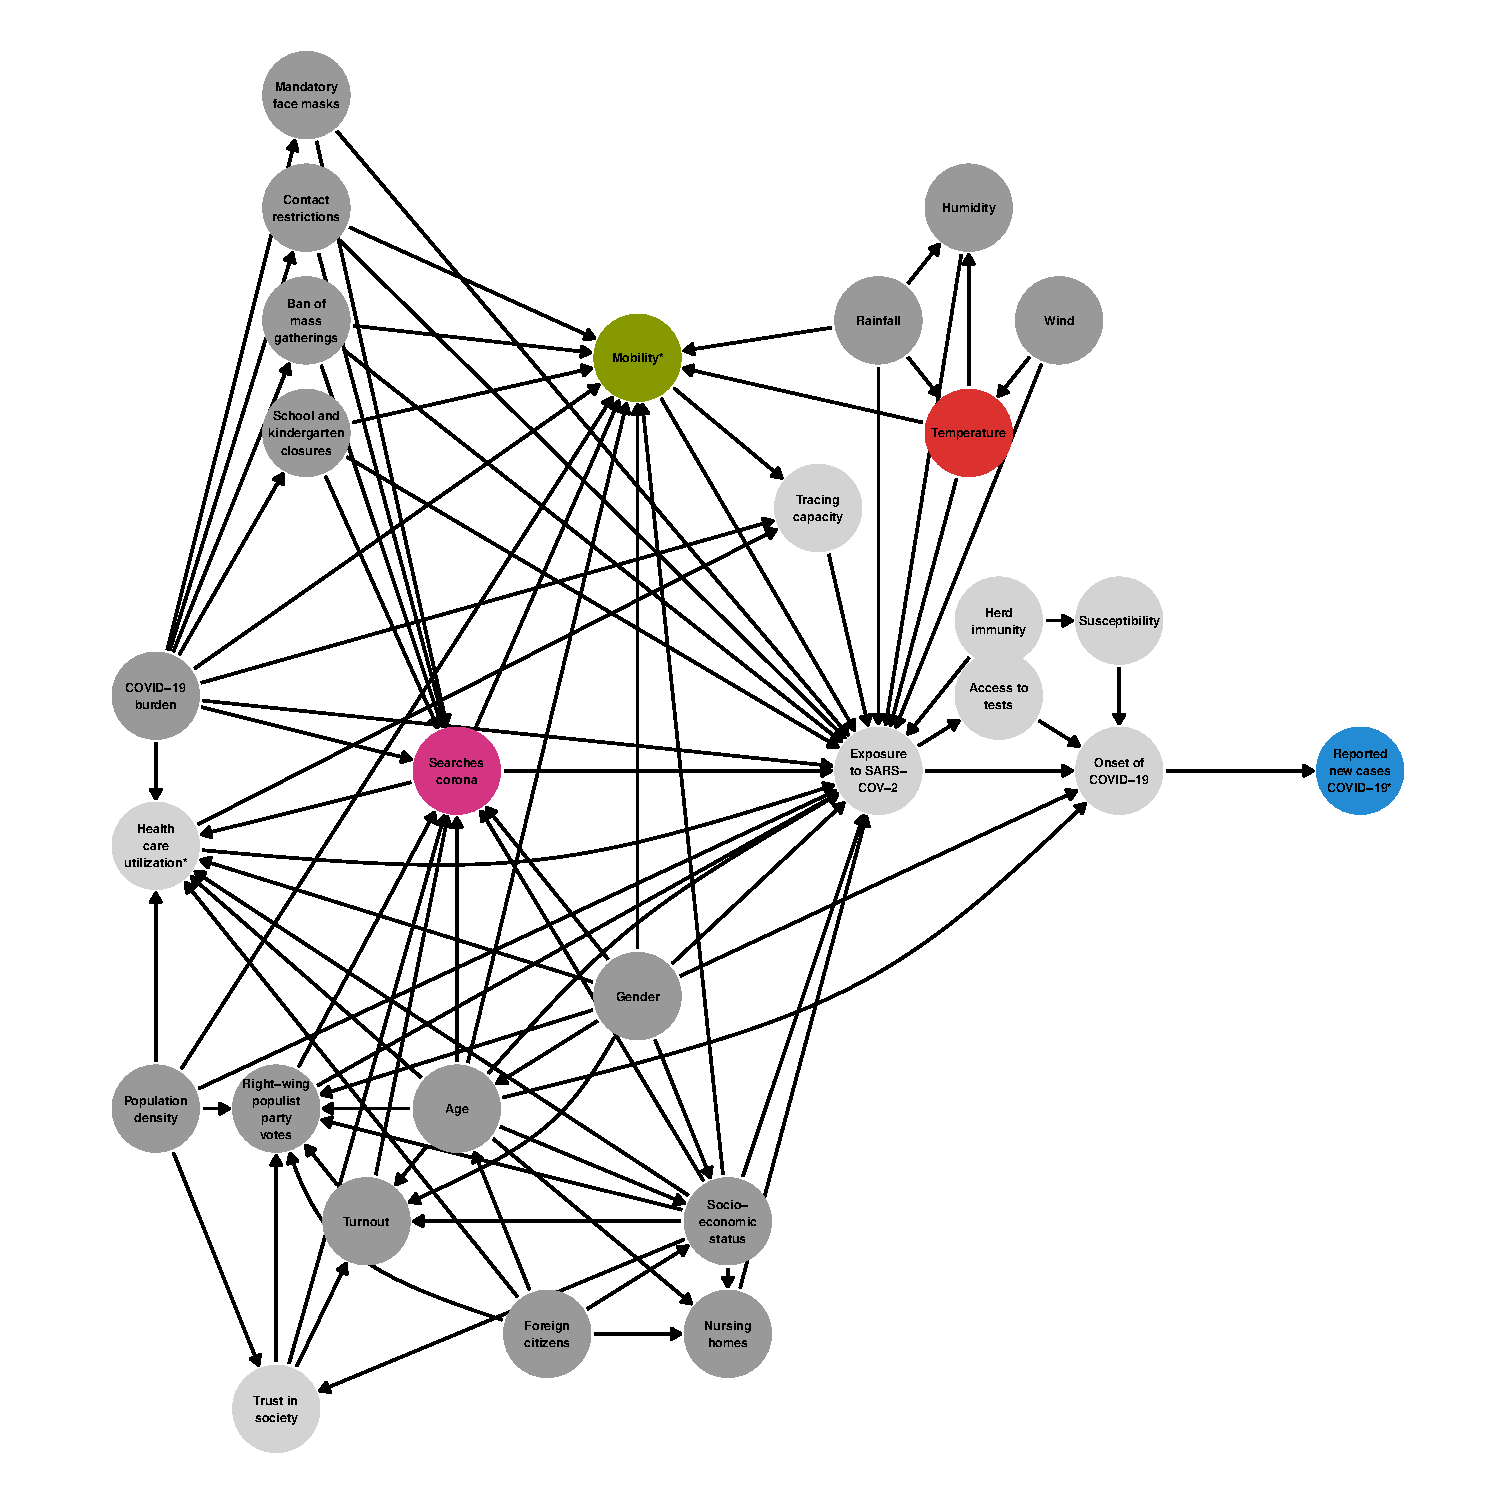
\includegraphics{figures/f_full_covid19_dag.eps}
%\caption{\label{fig:dag-covid-19}DAG of determinants of reported COVID-19
%cases on the district level. Unobserved variables are light gray,
%variables marked with an asterisk (*) are confounded by
%weekday/holiday.}
%\end{figure}

\begin{figure}[!h]
\caption{{\bf DAG of determinants of reported COVID-19 cases on the district level.}
Unobserved variables are light gray, variables marked with an asterisk (*) are confounded by weekday/holiday.}
\label{fig1}
\end{figure}

A number of studies report a strong association of \textbf{mobility}
restrictions on the number of new COVID-19 cases: Restrictive measures
(e.g. ``stay-at-home'' orders, travel bans, or school closures) are
shown to possibly reduce the COVID-19 incidence
\cite{chang_modeling_2020, Chinazzi395, fowler_effect_2020, kraemer_effect_2020, lasry_timing_2020, linka_outbreak_2020, mazzoli_effects_2020, xiong_data-driven_2020}.
However, some studies point out the combination of various
non-pharmaceutical interventions (NPIs) is decisive to prevent new
infections \cite{juni_impact_2020, lai_effect_2020}.

Google Trends \cite{google_trends} data can be used as a tool to get
insights into public interest (\textbf{awareness}) in the coronavirus
disease. Several recent studies imply a connection of relative search
volumes (RSV) indices and reported new COVID-19 cases
\cite{ayyoubzadeh_predicting_2020, effenberger_association_2020, higgins_correlations_2020, li_retrospective_2020, lin_google_2020, mavragani_tracking_2020, walker_use_2020, yuan_trends_2020, zhou_effects_2020}.
Some search terms e.g. ``COVID-19'' or ``coronavirus'' predated newly
infected cases/total number of cases by roughly 7 to 14 days for
different countries
\cite{effenberger_association_2020, higgins_correlations_2020, li_retrospective_2020, yuan_trends_2020}.
Additionally, we acknowledged that individual risk-aware behavior might
be a reaction to the current COVID-19 burden (measured as reported cases
at the day of exposure).

Mixed evidence is available regarding the effect of
\textbf{temperature}: On the one hand several papers report an
association between increase in temperature and decrease in newly
infected COVID-19 cases
\cite{bannister-tyrrell_preliminary_2020, demongeot_temperature_2020, liu_impact_2020, qi_covid-19_2020, shi_impact_2020, sobral_association_2020, tosepu_correlation_2020, Wang2020temperature, wu_effects_2020}.
On the other hand, also the opposite has been found
\cite{auler_evidence_2020, xie_association_2020}. Some studies found no
association at all
\cite{briz-redon_spatio-temporal_2020, iqbal_nexus_2020, jahangiri_sensitivity_2020, juni_impact_2020, yao_no_2020}.
It should be noted that few studies considered other confounding
variables than meteorological ones (especially age and population
density among others
\cite{briz-redon_spatio-temporal_2020, juni_impact_2020, wu_effects_2020}).
In addition, the transferability of results between different climate
zones is questionable. To avoid possible bias caused by weather
variables other than temperature, we included rain, wind, and humidity
in our model.

When investigating causal determinants of SARS-CoV-2 infections, a
number of confounders have to be considered. Well-known risk factors for
SARS-CoV-2 as well as for other infections are demographic factors such
as age, gender, socio-economic status (SES), population density, and
foreign citizenship/ethnicity
\cite{de2020risk, Dragano2020.06.17.20133918, jhucovid19db2020}. In
Germany along with other countries (i.e.~Brazil, USA, or the UK),
populist parties or politicians and their electorate tend to be more
sceptical about effects of containment measures than the other part of
the electorate \cite{dohle_wingen_schreiber_2020, engle_staying_2020}.
Therefore we considered both ``right-wing populist party votes'' and
``voter turnout'' as possible confounders. Public health interventions
were also taken into account (contact restrictions, school closures
etc.), as their implementation showed strong correlations with
controlling the spread of SARS-CoV-2
\cite{cowling2020impact, juni_impact_2020, lai_effect_2020}. To avoid
bias due to reporting delay of case numbers we had to include weekday
and German holidays. We included some unobserved variables in our DAG
(e.g.~``Herd immunity''), too. Please note that ``Exposure to
SARS-CoV-2'' is itself an unobserved variable: German case numbers are
reported with delay after date of exposure and symptom onset.
\emph{Exposure to the virus} should not be confused with the formal
\emph{exposure variables} of the DAG.

%Lorem ipsum dolor sit~\cite{bib1} amet, consectetur adipiscing elit. Curabitur eget porta erat. Morbi consectetur est vel gravida pretium. Suspendisse ut dui eu ante cursus gravida non sed sem. Nullam Eq~(\ref{eq:schemeP}) sapien tellus, commodo id velit id, eleifend volutpat quam. Phasellus mauris velit, dapibus finibus elementum vel, pulvinar non tellus. Nunc pellentesque pretium diam, quis maximus dolor faucibus id.~\cite{bib2} Nunc convallis sodales ante, ut ullamcorper est egestas vitae. Nam sit amet enim ultrices, ultrices elit pulvinar, volutpat risus.


%\begin{eqnarray}
%\label{eq:schemeP}
%	\mathrm{P_Y} = \underbrace{H(Y_n) - H(Y_n|\mathbf{V}^{Y}_{n})}_{S_Y} + \underbrace{H(Y_n|\mathbf{V}^{Y}_{n})- H(Y_n|\mathbf{V}^{X,Y}_{n})}_{T_{X\rightarrow Y}},
%\end{eqnarray}

\section*{Materials and methods}
\subsection*{Data}\label{data}

We collected and aggregated data on reported COVID-19 cases, regional
socio-demographic factors, weather, and general mobility on district and
state level in Germany for the period of 15 February 2020 to 8 July
2020. Our observation period for the outcome consisted of all dates from
20 February 2020 to 8 July 2020 (\(T=140\)), since we used a lag of 5
days for all confounders. We did not exclude any states or districts
(\(K=401\)). We analyzed the daily reported number of new cases as
outcome (\(K\cdot T=56{\ }140\) observations). The set of possible
predictors was derived from our causal DAG (see Table~\ref{tab:model-vars} and Fig~\ref{fig1}). Due to
modelling and data limitations, some of the predictors were unobserved
or were modelled as a construct consisting of several variables. For our causal graph analysis, we computed adjustment sets separately for all observed exposures within the DAG (if the respective exposure was identifiable within the DAG causal analysis framework).

\subsubsection*{Variables}\label{variables}

We downloaded German daily case numbers on district level reported by
Robert Koch Institute (RKI, \cite{casenumbers_rki}) and aggregated them by date. The number of daily active cases for
day \(d\) was derived by subtracting the total number of reported cases
on day \(d\) and day \(d-14\) (14 days as a conservative estimate for
the infectious period, which corresponds here to the required quarantine
time in Germany).

To assess the mobility of the German population, we used data publicly
available on German state level from Google \cite{google_mobility}.
Measurements are daily relative changes of mobility in percent compared
to the period of 3 January 2020 to 6 February 2020. Missing values
(\(25\) out of \(13{\ }488\)) were imputed with value \(0\) and the
state level measurements were passed onto districts within the
corresponding state. Google mobility data was available for six
different sectors of daily life (``retail and recreation'', ``grocery
and pharmacy'', ``parks'', ``transit stations'', ``workplaces'',
``residential'') which means that ``mobility'' is a construct consisting
of several variables. All variables but ``residential'' mobility are
relative changes of daily visitor numbers to the corresponding sectors
compared to the reference period. ``Residential'' mobility is the
relative change of daily time spent at residential areas. The six mobility variables showed high correlations among each other and with other variables. To reduce multicollinearity, we transformed them by principal component analysis (PCA) into six uncorrelated principal components which were used in place of the original variables.

The notion of awareness in the population of COVID-19 describes the
general state of alertness about the new infectious disease. As such, it
was hard to measure directly. As a proxy, we used the relative interest
in the topic term ``corona'' as indicated by Google searches. The daily
data was available on state level \cite{google_trends} and passed onto
district level. As a second proxy for awareness, we used the daily
reported number of COVID-19 cases on the day of the exposure: Since
media reported case numbers prominently, we assumed that this could
reflect individual awareness, too.

We constructed daily weather from four variables (``temperature'',
``rainfall'', ``humidity'', ``wind''). Weather data was downloaded from
Deutscher Wetterdienst (DWD, \cite{dwd_weather}) for all weather
stations in Germany below 1000 meters altitude with daily records for
our observation period. District level daily weather data was aggregated
per district by averaging the data from the three nearest weather
stations (which includes weather stations inside the district). Missing
values were imputed with mean values (\(n=59\) for wind).

The reported number of COVID-19 cases varied strongly by day of the
week. Thus, we included ``weekday'' as a categorical variable.
Similarly, the reported cases and the exposure to the virus were
affected by official holidays. Within the observation period, this
included among others Good Friday, Easter Monday, and Labor Day. To
correct for effects of these days, we included two variables in the
model, ``Holiday (report)'' (indicates if the day of the report was a
holiday, because governmental health departments were less likely to be
on full duty) and ``Holiday (exposure)'' (indicates if the day of
exposure to the virus was a holiday, because the population behaves
differently on holidays).

For different official and political interventions on a daily basis and the district level we used one-hot encoded daily variables, i.e.~ban of mass gatherings, school and kindergarten closures and their gradual reopening, contact restrictions, and mandatory face masks for shopping and public transport.

We included several social, economic, and demographic factors on the
district level with direct or indirect influence on the risk of exposure
to SARS-CoV-2 in our analysis. All are readily available from INKAR
database \cite{inkar}. We used the share of population that is 65 years
or older and the share of population that is younger than 18 years
(Age), the share of females in population (Gender), the population
density, the share of foreign citizenships and the share of the
population seeking refuge (Foreign citizenship), the share of low-income
households (Socio-economic status), voter turnout, share of right-wing
populist party votes, and the number of nursing (retirement) homes.

\begin{table}[!ht]
\begin{adjustwidth}{-2.25in}{0in} % Comment out/remove adjustwidth environment if table fits in text column.
\centering
\caption{
{\bf Observed model variables.}}
\fontsize{8}{10}\selectfont
\begin{tabular}[t]{llll>{\raggedright\arraybackslash}p{20em}l}
\toprule
variable & dynamics & level & type & unit/comment & source\\
\midrule
Weekday & daily & national & categorical & Sat through Thu as six binary variables, Fri as baseline & -\\
Holiday (report) & daily & national & binary & - & -\\
Holiday (exposure) & daily & national & binary & - & -\\
\addlinespace[0.3em]
\multicolumn{6}{l}{\textbf{Mobility}}\\
\hspace{1em}retail and recreation & daily & state & numeric & percent change compared to reference period & Google \cite{google_mobility}\\
\hspace{1em}grocery and pharmacy & daily & state & numeric & percent change compared to reference period & Google \cite{google_mobility}\\
\hspace{1em}parks & daily & state & numeric & percent change compared to reference period & Google \cite{google_mobility}\\
\hspace{1em}workplaces & daily & state & numeric & percent change compared to reference period & Google \cite{google_mobility}\\
\hspace{1em}residential & daily & state & numeric & percent change compared to reference period & Google \cite{google_mobility}\\
\hspace{1em}transit stations & daily & state & numeric & percent change compared to reference period & Google \cite{google_mobility}\\
\addlinespace[0.3em]
\multicolumn{6}{l}{\textbf{Awareness}}\\
\hspace{1em}Searches corona & daily & state & numeric & percent relative to other states and observation period & Google \cite{google_trends}\\
\hspace{1em}COVID-19 burden & daily & district & numeric & reported cases on day of exposure & RKI \cite{casenumbers_rki}\\
\addlinespace[0.3em]
\multicolumn{6}{l}{\textbf{Weather}}\\
\hspace{1em}Rainfall & daily & district & numeric & mm (l/sqm) & DWD \cite{dwd_weather}\\
\hspace{1em}Temperature & daily & district & numeric & °C & DWD \cite{dwd_weather}\\
\hspace{1em}Humidity & daily & district & numeric & relative humidity (\%) & DWD \cite{dwd_weather}\\
\hspace{1em}Wind & daily & district & numeric & m/s & DWD \cite{dwd_weather}\\
\addlinespace[0.3em]
\multicolumn{6}{l}{\textbf{Interventions}}\\
\hspace{1em}Ban of mass gatherings & daily & national & binary & - & -\\
\hspace{1em}School and kindergarten closures & daily & state & numeric & 0 for no closure, 1 for full closure, 0.5 for partial reopening & -\\
\hspace{1em}Contact restrictions & daily & national & binary & - & -\\
\hspace{1em}Mandatory face masks & daily & district & binary & - & IZA \cite{mitze2020face}\\
\addlinespace[0.3em]
\multicolumn{6}{l}{\textbf{Socio-demographic}}\\
\hspace{1em}Age & constant & district & numeric & 2 variables: share of population >=65 years \& <18 years & INKAR \cite{inkar}\\
\hspace{1em}Gender & constant & district & numeric & share of female population & INKAR \cite{inkar}\\
\hspace{1em}Population density & constant & district & numeric & population per sqkm & INKAR \cite{inkar}\\
\hspace{1em}Foreign citizens & constant & district & numeric & 2 variables: share of foreign citizens \& of population seeking refuge & INKAR \cite{inkar}\\
\hspace{1em}Socio-economic status & constant & district & numeric & share of households with low income & INKAR \cite{inkar}\\
\hspace{1em}Turnout & constant & district & numeric & voter turnout in last election & INKAR \cite{inkar}\\
\hspace{1em}Right-wing populist party votes & constant & district & numeric & share of votes for AfD in last election & INKAR \cite{inkar}\\
\hspace{1em}Nursing homes & constant & district & numeric & number of nursing (retirement) homes & INKAR \cite{inkar}\\
\addlinespace[0.3em]
\multicolumn{6}{l}{\textbf{Case numbers}}\\
\hspace{1em}Reported new cases of COVID-19 & daily & district & numeric & - & RKI \cite{casenumbers_rki}\\
\hspace{1em}Active cases & daily & district & numeric & active cases on day of report & RKI \cite{casenumbers_rki}\\
\bottomrule
\end{tabular}
\label{tab:model-vars}
\end{adjustwidth}
\end{table}

All continuous variables but the outcome ``Reported new cases of COVID-19'' and the offset ``Active cases'' were centered and scaled by one standard deviation for numerical stability, while we left binary variables as-is. After estimating the effects of variables, we re-scaled continuous variables' effects to their original scale. Additionally for mobility variables, we re-transformed the effects of the principal components to the original mobility variables. Furthermore, we lagged the effect of all variables (but outcome, offset, and the non-dynamic socio-demographic variables) by 5 days (optimal lag found by cross-validation) which means that we assumed that their effects on the outcome will be visible after 5 days.

\subsection*{Methods}\label{methods}

\subsubsection*{Causal analysis with DAG and adjustment
sets}\label{causal-analysis-with-dag-and-adjustment-sets}

We used a directed acyclic graph as a graphical representation of the
hypothesized causal reasoning that leads to exposure to the SARS-CoV-2
virus, onset of COVID-19, and finally reports of COVID-19 cases. We use the terms ``causal effect'' or ``causal relationship'' for effect estimates that are based on this causal graph framework. Every
node \(v_i\) in the graph is the graphical representation of an observed
or unobserved variable \(x_i\), a directed edge \(e_{ij}\) is an arrow
from node \(v_i\) to \(v_j\) that implies a direct causal relationship
from variable \(x_i\) onto variable \(x_j\). The set of all nodes is
denoted by \(V\), the set of all edges by \(E\), as such, the complete
DAG is the tuple \(G=(V,E)\). The seminal works of Spirtes and Pearl
\cite{spirtes2000causation, pearl2009causality} introduce the theory of
causal analysis, do-calculus, and how to analyze a DAG to estimate the
total or direct causal effect from a variable \(x_i\) onto a variable
\(x_j\). The direct effect is the effect associated with the edge
\(e_{ij}\) only (if it exists), while the total effect takes indirect
effects via other paths from \(v_i\) to \(v_j\) into account, too. Here
we estimated total effects only, since most of our variables were not
hypothesized to have a direct effect on the \emph{reported} number of
new COVID-19 cases. In contrast to prediction tasks, where one would
include all variables available, it is actually ill-advised to use all
available variables to estimate causal effects, due to introducing bias
by adjusting for unnecessary variables within the causal DAG. This is
why we need to identify a valid set of necessary variables (an
adjustment set) to estimate the proper causal effect
\cite{pearl2009causality}. The ``minimal adjustment set''
\cite{greenland1999causal} is a valid adjustment set of variables that
does not contain another valid adjustment set as a subset. However,
identifying a minimal adjustment set might not be enough to reliably
estimate the causal effect. Thus, we identified the ``optimal adjustment
set'' \cite{henckel2019graphical} as the set of variables which is a
valid adjustment set while having the lowest Akaike information criterion (AIC).

We analyzed the DAG from Fig~\ref{fig1} with the R Software
\cite{rsoftware} and the R packages \texttt{dagitty} (formal
representation of the graph and minimal adjustment sets
\cite{textor_robust_2017}) and \texttt{pcalg} (for finding an optimal
adjustment set \cite{pcalg}). For the defined exposures and the outcome
``Reported new cases of COVID-19'', we computed the minimal and optimal
adjustment sets. Since it was possible that these sets contained unobserved variables that needed to be left out of the regression model, we chose the valid set with the lowest AIC (see next section) to estimate the final total causal effect from exposure to outcome.

\subsubsection*{Regression with negative binomial
model}\label{regression-with-negative-binomial-model}

We can estimate the causal effect from exposure to outcome by regression
\cite{pearl2009causality}. Since the outcome ``Reported new cases of
COVID-19'' is a count variable, one should not employ a linear
regression model with Gaussian errors, but instead we assumed a
log-linear relationship between the expected value of the outcome \(Y\)
(new cases) and regressors \(x\), as well as a Poisson or negative
binomial distribution for \(Y\):

\begin{equation}
\log(\mathbb{E}[Y|x]) = \alpha + \sum_{i\in S}\beta_i\cdot x_{i}, \label{eq:regmodel}
\end{equation}

where \(\alpha\) is the regression intercept, \(S\) is the set of
adjustment variables for the exposure \(i^{\ast}\) including the
exposure variable itself, \(\beta_i\) are the regression coefficients
corresponding to the variables \(x_i\). As such \(\beta_{i^{\ast}}\) is
the total causal effect from exposure variable \(x_{i^{\ast}}\) on the
outcome Y.

The Poisson regression assumes equality of mean and variance. If this is
not the case one observes so-called overdispersion (the variance is
higher than the mean), this indicates one should use regression with a
negative binomial distribution instead to estimate the variance
parameter separately from the mean.

We needed to account for the fact that our outcome is not counted per
time unit (one day) only, but depends on the number of active COVID-19
cases: Holding all other variables fixed, the number of new cases \(Y\)
is a constant proportion of the number of active cases \(A\). This was
modeled by including an offset \(\log(A+1)\) in the regression model Eq~\eqref{eq:regmodel}:

\begin{align}
\log(\mathbb{E}[Y|x]) &= \alpha + \log(A+1) + \sum_{i\in S}\beta_i\cdot x_{i} \nonumber \\
\Leftrightarrow \log(\frac{\mathbb{E}[Y|x]}{A+1}) &= \alpha + \sum\beta_i\cdot x_{i} \label{eq:logratemodel} \\
\Leftrightarrow \frac{\mathbb{E}[Y|x]}{A+1} &= \exp(\alpha)\cdot \prod \exp(\beta_i)^{x_i}. \label{eq:ratechange}
\end{align}

Here we added a pseudocount ``\(+1\)'' to ensure a finite logarithm and
avoid division by \(0\).

One can interpret the model as approximating the log-ratio of new cases
and active cases by a linear combination of the regressor variables in Eq~\eqref{eq:logratemodel}. If all variables \(x_i\) are centered in Eq~\eqref{eq:ratechange}, we have for the baseline
\(\forall i\ x_i=0 \Rightarrow \mathbb{E}[Y|x=0]=\exp(\alpha)\cdot (A+1)\).
In other words, the exponentiated intercept is the baseline daily
infection rate (how many people does one infected individual infect in
one day). If we hold all variables \(x_i\) fixed (e.g.~at baseline 0) in Eq~\eqref{eq:ratechange} but now increase the exposure variable
\(x_{i^{\ast}}=0\) by one unit to \(x_{i^{\ast}}+1=0+1\), we have
\begin{align*}
\mathbb{E}[Y|x']&=\exp(\alpha)\cdot(A+1)\cdot\exp(\beta_{i^{\ast}}^{x_{i^{\ast}}+1})\prod_{i\neq i^{\ast}}\exp(\beta_i)^0 \\
&=\exp(\alpha)\cdot(A+1)\cdot\exp(\beta_{i^{\ast}}),
\end{align*}
which means the exponentiated coefficient \(\beta_{i^{\ast}}\) describes
the rate change of the outcome by one unit increase of the exposure.

In practice, given observations of \(Y\) and \(x\) we estimate the
regression coefficients \(\alpha\) and \(\beta_i\) by maximum
likelihood \cite{maxlikelihood}. Our observational measurements are
\(y_{kt}\) and \(x_{ikt}\), where \(k\) indicates the corresponding
district and \(t\) the date of measurement.

We conducted a log-linear regression (function \texttt{glm} with \texttt{family=poisson()} for Poisson regression, and \texttt{glm.nb} from the \texttt{MASS} package for the negative binomial regression \cite{mass}) for the full data set to assess general model adequacy and to estimate the \(\theta\) parameter of the negative binomial. The proper lag between exposures and outcome was found by 10-fold cross-validation on different lags between 1 and 20 days. Model diagnostics on the final full model did not show severe problems with model assumptions (linearity, distribution of residuals, independence of observations). Analysis of variance inflation factors revealed some problems with multicollinearity. To reduce the effects of multicollinearity, first we transformed the highly correlated mobility variables by PCA as described above. Second, we used a ridge regression approach \cite{ridge1970}, which is a regularization method that shrinks regression coefficients and alleviates the effect of correlation between variables on their respective regression coefficients. Furthermore, regularized regression allows for better fits on unseen data, thus preventing overfitting the data, too. The hyper-parameter \(\lambda\) of the ridge regression was chosen by 10-fold cross-validation, where the folds were constructed from random subsets of the \(401\) districts. We used this hyper-parameter with the \texttt{cv.glmnet} function from the R package \texttt{glmnet} \cite{glmnet2010} with \texttt{family=negative.binomial(theta)} and chose the \(\lambda\) value within one standard deviation from the minimal \(\lambda\) as regularization hyper-parameter. Afterwards, we calculated the effects of separate exposures on the outcome. For every exposure, we analyzed the different valid adjustment sets given by analysis of the causal DAG (i.e.~the minimal and optimal adjustment sets). Then, we first checked if the respective set included unobserved variables. If this was the case for the optimal adjustment set, we discarded the unobserved variables from the set and checked if it was still a valid adjustment set (function \texttt{gac} in package \texttt{pcalg} \cite{perkovi2015complete}). If a minimal adjustment set contained unobserved variables, we discarded the whole set. If no valid adjustment set for a given exposure was available, we concluded that the effect of this exposure was unidentifiable within our causal graph. We used the function \texttt{glmnet} with the parameters \(\theta\) and \(\lambda\) as above on every remaining valid adjustment set as regressors (that is, we applied ridge regression) and calculated the Akaike information criterion (AIC) for this model/set of regressors. Finally, for every exposure, we decided for the model/adjustment set (if available) with the lowest AIC. We report the exponentiated estimated coefficients for the separate exposures on their original scale.

%% For figure citations, please use "Fig" instead of "Figure".
%Nulla mi mi, Fig~\ref{fig1} venenatis sed ipsum varius, volutpat euismod diam. Proin rutrum vel massa non gravida. Quisque tempor sem et dignissim rutrum. Lorem ipsum dolor sit amet, consectetur adipiscing elit. Morbi at justo vitae nulla elementum commodo eu id massa. In vitae diam ac augue semper tincidunt eu ut eros. Fusce fringilla erat porttitor lectus cursus, \nameref{S1_Video} vel sagittis arcu lobortis. Aliquam in enim semper, aliquam massa id, cursus neque. Praesent faucibus semper libero.
%
%% Place figure captions after the first paragraph in which they are cited.
%\begin{figure}[!h]
%\caption{{\bf Bold the figure title.}
%Figure caption text here, please use this space for the figure panel descriptions instead of using subfigure commands. A: Lorem ipsum dolor sit amet. B: Consectetur adipiscing elit.}
%\label{fig1}
%\end{figure}

% Results and Discussion can be combined.
\section*{Results}\label{results}

Descriptive statistics for the included variables are presented in Table~\ref{tab:descriptive-vars}.

\begin{table}[!ht]
%\begin{adjustwidth}{-2.25in}{0in} % Comment out/remove adjustwidth environment if table fits in text column.
\centering
\caption{
{\bf Descriptive statistics for observed variables.}}
%\fontsize{8}{10}\selectfont
\begin{tabular}[t]{ll}
\toprule
Variable & mean (SD)\\
\midrule
n & 56140\\
\addlinespace[0.3em]
\multicolumn{2}{l}{\textbf{Mobility}}\\
\hspace{1em}retail and recreation & -26.62 (24.60)\\
\hspace{1em}grocery and pharmacy & -3.94 (22.77)\\
\hspace{1em}parks & 47.26 (58.20)\\
\hspace{1em}workplaces & -22.96 (20.35)\\
\hspace{1em}residential & 8.13 (6.49)\\
\hspace{1em}transit stations & -29.58 (21.11)\\
\addlinespace[0.3em]
\multicolumn{2}{l}{\textbf{Awareness}}\\
\hspace{1em}Searches corona & 26.94 (18.23)\\
\hspace{1em}COVID-19 burden & 3.50 (10.28)\\
\addlinespace[0.3em]
\multicolumn{2}{l}{\textbf{Weather}}\\
\hspace{1em}Rainfall & 1.89 (4.01)\\
\hspace{1em}Temperature & 10.90 (5.33)\\
\hspace{1em}Humidity & 67.81 (13.03)\\
\hspace{1em}Wind & 3.63 (1.66)\\
\addlinespace[0.3em]
\multicolumn{2}{l}{\textbf{Interventions}}\\
\hspace{1em}Ban of mass gatherings & 0.83 (0.38)\\
\hspace{1em}School and kindergarten closures & 0.54 (0.36)\\
\hspace{1em}Contact restrictions & 0.74 (0.44)\\
\hspace{1em}Mandatory face masks & 0.49 (0.50)\\
\addlinespace[0.3em]
\multicolumn{2}{l}{\textbf{Socio-demographic}}\\
\hspace{1em}Age (pop. 65 and older) & 22.09 (2.74)\\
\hspace{1em}Age (pop. younger 18) & 16.17 (1.25)\\
\hspace{1em}Gender & 50.59 (0.64)\\
\hspace{1em}Population density & 533.75 (701.84)\\
\hspace{1em}Foreign citizens & 10.03 (5.14)\\
\hspace{1em}Foreign citizens (refugees) & 1.88 (1.14)\\
\hspace{1em}Socio-economic status & 30.64 (6.02)\\
\hspace{1em}Turnout & 75.08 (3.79)\\
\hspace{1em}Right-wing populist party votes & 13.39 (5.32)\\
\hspace{1em}Nursing homes & 36.11 (30.69)\\
\addlinespace[0.3em]
\multicolumn{2}{l}{\textbf{Case numbers (Outcome and offset)}}\\
\hspace{1em}Reported new cases COVID-19 & 3.53 (10.29)\\
\hspace{1em}Active cases & 48.76 (120.86)\\
\bottomrule
\end{tabular}
\label{tab:descriptive-vars}
%\end{adjustwidth}
\end{table}

In the observational period, the number of daily reported COVID-19 cases increased till the end of March/beginning of April and continually decreased afterwards till the beginning of June 2020 with a slight increase and decrease afterwards (Fig~\ref{fig2}A). On the other hand, the (log-)ratio of reported cases over active cases decreased steeply till the mid of April and increased steadily afterwards with a slight decrease close to the end of the observation period (Fig~\ref{fig2}B). Both figures examplify a considerable variation among the districts (light blue points are individual district's data).

\begin{figure}[!h]
\caption{{\bf Temporal and district level variation of outcome (log-scale).}}
\label{fig2}
\end{figure}

In Germany, we observed a rebound in mobility after the initial political measures, reductions in incident cases were associated with a diminishing public interest in COVID-19, and temperatures were overall increasing (cf.~Fig~\ref{fig3}); with correlations between temporal progression and mobility in retail and recreation \(r_{A,B}=\) 0.02, awareness (``Searches corona'') \(r_{A,C}=\) -0.3, and temperature \(r_{A,D}=\) 0.8.

\begin{figure}[!h]
\caption{{\bf Temporal variation of outcome and main
determinants.}}
\label{fig3}
\end{figure}

\subsection*{Main results}\label{main-results}

We list the results of our causal analysis for the effects of different exposure variables in Table~\ref{tab:causaleffects}. The estimates are multiplicative rates of increase/decrease for a one unit increase of the respective variable: Values above 1 lead to an increase, below 1 to a decrease of the infection rate. To put these estimates into perspective, Fig~\ref{fig4} shows the relative causal effect of the different exposure variables on the number of reported COVID-19 cases on a range of sensible values of the exposure variables (95 percent quantiles of data points).

\begin{table}[!ht]
%\begin{adjustwidth}{-2.25in}{0in} % Comment out/remove adjustwidth environment if table fits in text column.
\centering
\caption{
{\bf Effect estimates from causal graph analysis.}}
%\fontsize{8}{10}\selectfont
\begin{tabular}[t]{lr}
\toprule
cause & effect estimate\\
\midrule
\addlinespace[0.3em]
\multicolumn{2}{l}{\textbf{Mobility}}\\
\hspace{1em}retail and recreation & 1.0011\\
\hspace{1em}grocery and pharmacy & 0.9977\\
\hspace{1em}parks & 0.9997\\
\hspace{1em}transit stations & 1.0026\\
\hspace{1em}workplaces & 1.0033\\
\hspace{1em}residential & 0.9903\\
\addlinespace[0.3em]
\multicolumn{2}{l}{\textbf{Awareness}}\\
\hspace{1em}Searches corona & 1.0089\\
\hspace{1em}COVID-19 burden & 0.9980\\
\addlinespace[0.3em]
\multicolumn{2}{l}{\textbf{Weather}}\\
\hspace{1em}Temperature & 0.9905\\
\hspace{1em}Rainfall & 1.0121\\
\hspace{1em}Humidity & 1.0057\\
\hspace{1em}Wind & 1.0329\\
\addlinespace[0.3em]
\multicolumn{2}{l}{\textbf{Interventions}}\\
\hspace{1em}Interventions (ban of mass gatherings) & 0.9729\\
\hspace{1em}Interventions (school and kindergarten closures) & 0.9277\\
\hspace{1em}Interventions (contact restrictions) & 0.8314\\
\hspace{1em}Interventions (mandatory face masks) & 0.9064\\
\addlinespace[0.3em]
\multicolumn{2}{l}{\textbf{Demographic}}\\
\hspace{1em}Age (pop. 65 and older) & 0.9953\\
\hspace{1em}Age (pop. younger 18) & 1.0120\\
\hspace{1em}Foreign citizens & 1.0048\\
\hspace{1em}Foreign citizens (refugees) & 0.9985\\
\hspace{1em}Gender & 0.9925\\
\hspace{1em}Nursing homes & 1.0011\\
\hspace{1em}Population density & 1.0000\\
\hspace{1em}Socio-economic status & 0.9982\\
\bottomrule
\end{tabular}
\label{tab:causaleffects}
%\end{adjustwidth}
\end{table}

\begin{figure}[!h]
\caption{{\bf Relative causal effects of exposures.}}
\label{fig4}
\end{figure}

Within our framework, we saw very different effects for individual mobility variables. For mobility in retail/recreation, an increase of 1 percent point mobility compared to the reference period (03 January to 06 February 2020) leads to an increase of the daily reported case number by about 0.11 percent. Similarly, mobility on workplaces showed an effect of 0.33 increase in case numbers for every 1 percent point increase in mobility, while mobility on transit stations showed an effect of 0.26 increase in case numbers for every 1 percent point increase. Contrarily, the remaining three mobility variables showed negative effects on the number of reported COVID-19 cases. An increase of 1 percent point mobility for the areas of grocery/pharmacy leads to a decrease in the reported case number by approximately 0.23 percent, while increased mobility of 1 percent point within parks leads to a decrease in the reported case number by approximately 0.03 percent, and finally an increase of 1 percent point in residential mobility leads to a decrease by approximately 0.97 percent. Fig~\ref{fig4} shows the effects of mobility on a range of possible values. Thus, we expect an increase of daily cases by approximately 7.8 percent if mobility in workplaces reaches baseline levels of 0 percent difference to the reference period. On the other hand, an increase of mobility for residential areas by 10 percent points compared to the reference period leads to a reduction of the infection rate by approximately 1.8 percent.

``Awareness'' had two opposite effects on the outcome in our DAG. Awareness measured by Google searches for \emph{corona} had a positive effect on the number of reported cases. An one percent point increase of the state's Google searches (relative to other states and the observation period) leads to an increase of approximately 0.89 percent. For example, if a district shows 10 percent points more relative searches for \emph{corona} than another one, we expect approximately 9.3 percent more infections for this district after 5 days. \emph{COVID-19 burden} (reported number of cases on day of exposure) affected the outcome negatively, where every additional daily case in the district leads to a 0.2 percent decrease in newly reported case numbers. The corresponding plot in Fig~\ref{fig4} visualizes this relationship: For a local outbreak with 20 daily cases as COVID-19 burden, we estimate as total causal effect a subsequent reduction of infection rate by 3.9 percent.

Within our model, we observed effects of temperature and all other weather variables. Every increase of 1 degree Celsius in temperature leads to a reduction of the daily reported case numbers by approximately 0.95 percent. On the other hand, we found an increasing effect of rainfall: One millimeter (=1 liter per square meter) more rainfall leads to an increase of reported case numbers by approximately 1.21 percent. We observe effects for humidity and wind as well (higher humidity and stronger wind leading to more cases). In perspective (Fig~\ref{fig4}), with temperature we expect an increase by approximately 21 percent at a daily average temperature of \(0^{\circ}C\) compared to a day with \(20^{\circ}C\). For rainfall, we expect on a rainy day with 10 mm rainfall a corresponding increase of the infection rate by approximately 12.8 percent compared to a day with no precipitation.

The different intervention variables showed the strongest effects in our analysis, see Table~\ref{tab:causaleffects}. While the first intervention (ban of mass gatherings) reduced subsequent daily case numbers by 2.7 percent, the closure of schools/kindergartens reduced infections by an additional 7.2 percent and mandatory face masks reduced this by another 9.4 percent. The effect of contact restrictions was the strongest in our observation period, with an reduction of the case rates by 16.9.

The effects of the different socio-demographic factors are quite small in comparison to the effects described above. We see an increasing effect on case numbers by additional nursing homes between districts. Districts with a younger population, more foreign citizens, higher population density and a lower average social-economic status showed higher case numbers, too.

For all exposures, our analysis pipeline opted to use the (reduced) optimal adjustment set over the minimal adjustment sets because of lower AICs, except for exposure variable ``nursing homes'', for which the minimal adjustment set had the lowest AIC. For an overview of all final adjustments sets, see Table~\ref{tab:adjsets}. We found that there were no valid adjustment sets for the non-identifiable variables turnout and right-wing populist party votes.

We decided for a lag of 5 days based on cross-validation. Similarly, negative binomial regression was chosen over Poisson regression, because the latter showed overdispersion and an higher AIC value.

\begin{table}[!ht]
\begin{adjustwidth}{-2.25in}{0in} % Comment out/remove adjustwidth environment if table fits in text column.
\centering
\caption{
{\bf Final adjustment sets for causal analysis.}}
%\fontsize{8}{10}\selectfont
\begin{tabular}[t]{lllllllllllllll}
\toprule
\rotatebox{90}{ } & \rotatebox{90}{Mobility} & \rotatebox{90}{Searches corona} & \rotatebox{90}{COVID-19 burden} & \rotatebox{90}{Temperature} & \rotatebox{90}{Rainfall} & \rotatebox{90}{Humidity} & \rotatebox{90}{Wind} & \rotatebox{90}{Interventions} & \rotatebox{90}{Age} & \rotatebox{90}{Foreign citizens} & \rotatebox{90}{Gender} & \rotatebox{90}{Nursing homes} & \rotatebox{90}{Population density} & \rotatebox{90}{Socio-economic status}\\
\midrule
Weekday & x & x & x & x & x & x & x & x & x & x & x & x & x & x\\
Holiday (report) & x & x & x & x & x & x & x & x & x & x & x & x & x & x\\
Holiday (exposure) & x & x & x & x & x & x & x & x & x & x & x & x & x & x\\
\addlinespace[0.3em]
\multicolumn{15}{l}{\textbf{Mobility}}\\
\hspace{1em}Mobility &  &  &  &  &  & x &  &  &  &  &  &  &  & \\
\addlinespace[0.3em]
\multicolumn{15}{l}{\textbf{Awareness}}\\
\hspace{1em}Searches corona & x &  &  & x & x & x & x &  &  &  &  & x &  & \\
\hspace{1em}COVID-19 burden & x & x &  & x & x & x & x & x & x & x & x & x & x & x\\
\addlinespace[0.3em]
\multicolumn{15}{l}{\textbf{Weather}}\\
\hspace{1em}Temperature & x & x & x &  &  & x &  & x & x & x & x &  & x & x\\
\hspace{1em}Rainfall & x & x & x & x &  & x & x & x & x & x & x &  & x & x\\
\hspace{1em}Humidity & x & x & x &  &  &  &  & x & x & x & x &  & x & x\\
\hspace{1em}Wind & x & x & x & x & x & x &  & x & x & x & x &  & x & x\\
\addlinespace[0.3em]
\multicolumn{15}{l}{\textbf{Interventions}}\\
\hspace{1em}Interventions & x & x &  & x & x & x & x &  & x & x & x & x & x & x\\
\addlinespace[0.3em]
\multicolumn{15}{l}{\textbf{Socio-demographic}}\\
\hspace{1em}Age & x & x & x & x & x & x & x & x &  &  &  & x & x & x\\
\hspace{1em}Gender & x & x & x & x & x & x & x & x & x & x &  & x & x & x\\
\hspace{1em}Population density & x & x & x & x & x & x & x & x & x & x & x & x &  & x\\
\hspace{1em}Foreign citizens &  & x & x &  &  &  &  & x & x &  & x &  & x & x\\
\hspace{1em}Socio-economic status & x & x & x & x & x & x & x & x &  &  &  & x & x & \\
\hspace{1em}Turnout &  &  & x &  &  &  &  & x &  &  &  &  &  & \\
\hspace{1em}Right-wing populist party votes & x & x & x & x & x & x & x & x &  &  &  & x &  & \\
\hspace{1em}Nursing homes & x & x & x & x & x & x & x & x &  &  &  &  & x & \\
\bottomrule
\end{tabular}
\label{tab:adjsets}
\end{adjustwidth}
\end{table}

%Nulla mi mi, venenatis sed ipsum varius, Table~\ref{table1} volutpat euismod diam. Proin rutrum vel massa non gravida. Quisque tempor sem et dignissim rutrum. Lorem ipsum dolor sit amet, consectetur adipiscing elit. Morbi at justo vitae nulla elementum commodo eu id massa. In vitae diam ac augue semper tincidunt eu ut eros. Fusce fringilla erat porttitor lectus cursus, vel sagittis arcu lobortis. Aliquam in enim semper, aliquam massa id, cursus neque. Praesent faucibus semper libero.

%% Place tables after the first paragraph in which they are cited.
%\begin{table}[!ht]
%\begin{adjustwidth}{-2.25in}{0in} % Comment out/remove adjustwidth environment if table fits in text column.
%\centering
%\caption{
%{\bf Table caption Nulla mi mi, venenatis sed ipsum varius, volutpat euismod diam.}}
%\begin{tabular}{|l+l|l|l|l|l|l|l|}
%\hline
%\multicolumn{4}{|l|}{\bf Heading1} & \multicolumn{4}{|l|}{\bf Heading2}\\ \thickhline
%$cell1 row1$ & cell2 row 1 & cell3 row 1 & cell4 row 1 & cell5 row 1 & cell6 row 1 & cell7 row 1 & cell8 row 1\\ \hline
%$cell1 row2$ & cell2 row 2 & cell3 row 2 & cell4 row 2 & cell5 row 2 & cell6 row 2 & cell7 row 2 & cell8 row 2\\ \hline
%$cell1 row3$ & cell2 row 3 & cell3 row 3 & cell4 row 3 & cell5 row 3 & cell6 row 3 & cell7 row 3 & cell8 row 3\\ \hline
%\end{tabular}
%\begin{flushleft} Table notes Phasellus venenatis, tortor nec vestibulum mattis, massa tortor interdum felis, nec pellentesque metus tortor nec nisl. Ut ornare mauris tellus, vel dapibus arcu suscipit sed.
%\end{flushleft}
%\label{table1}
%\end{adjustwidth}
%\end{table}

%%PLOS does not support heading levels beyond the 3rd (no 4th level headings).
%\subsection*{\lorem\ and \ipsum\ nunc blandit a tortor}
%\subsubsection*{3rd level heading} 
%Maecenas convallis mauris sit amet sem ultrices gravida. Etiam eget sapien nibh. Sed ac ipsum eget enim egestas ullamcorper nec euismod ligula. Curabitur fringilla pulvinar lectus consectetur pellentesque. Quisque augue sem, tincidunt sit amet feugiat eget, ullamcorper sed velit. Sed non aliquet felis. Lorem ipsum dolor sit amet, consectetur adipiscing elit. Mauris commodo justo ac dui pretium imperdiet. Sed suscipit iaculis mi at feugiat. 
%
%\begin{enumerate}
%	\item{react}
%	\item{diffuse free particles}
%	\item{increment time by dt and go to 1}
%\end{enumerate}
%
%
%\subsection*{Sed ac quam id nisi malesuada congue}
%
%Nulla mi mi, venenatis sed ipsum varius, volutpat euismod diam. Proin rutrum vel massa non gravida. Quisque tempor sem et dignissim rutrum. Lorem ipsum dolor sit amet, consectetur adipiscing elit. Morbi at justo vitae nulla elementum commodo eu id massa. In vitae diam ac augue semper tincidunt eu ut eros. Fusce fringilla erat porttitor lectus cursus, vel sagittis arcu lobortis. Aliquam in enim semper, aliquam massa id, cursus neque. Praesent faucibus semper libero.
%
%\begin{itemize}
%	\item First bulleted item.
%	\item Second bulleted item.
%	\item Third bulleted item.
%\end{itemize}

\section*{Discussion}\label{discussion}

\subsection*{Main findings}\label{main-findings}

Our objective was to identify effects of determining factors for COVID-19 cases within a causal framework. We found that weather affects the reported number of infections, especially temperature (which has a reducing effect on case numbers) and rainfall (which increases case numbers). We saw that reports of high case numbers in districts led to a reduction in new infection numbers, which indicates risk-averse awareness in the population and/or effective public health measures to suppress a local outbreak. Mobility showed distinct effects: Increasing activity in retail and recreational areas, as well as transit stations and workplaces increased reported case numbers, while increased movement for essential shopping (grocery and pharmacy) and in parks or residential areas led to reduced case numbers. All interventions considered (ban of mass gatherings, school/kindergarten closures, contact restrictions, mandatory face masks) reduced case numbers considerably. Socio-demographic variables had small effects individually, but in conjunction they explained larger case numbers in (urban) areas with younger population, lower socio-economic status, and higher population density.

Furthermore, we made a strong case for the use of causal DAGs in epidemiology and a pandemic like COVID-19: DAGs allow to choose confounders for the analysis in a principled and statistically correct way while reducing possible causes for bias. Also, the DAG formalization allows for discussion about the underlying causal assumptions.

\subsection*{Comparison with previous
research}\label{comparison-with-previous-research}

Most research on determinants affecting case numbers of COVID-19 is restricted to single aspects \cite{fowler_effect_2020, li_retrospective_2020, shi_impact_2020, Wang2020temperature}. To reliably identify (causal) drivers, one must adjust for confounders. To this end, we used an integrated model with variables from different aspects like mobility, awareness, weather, or socio-demographics and identified confounders by causal analysis with a directed acyclic graph. A causal approach is used in another current COVID-19 analysis \cite{gencoglu2020causal}. There, however, they identify the causal relationships (reconstruct a DAG), while we estimated effects for a given hypothesized causal DAG.

Several studies assessing the impact of public health measures on mobility have each observed a downward trend accompanied by a decrease in the number of newly reported cases \cite{chang_modeling_2020, cowling2020impact, fowler_effect_2020, kraemer_effect_2020, lai_effect_2020, linka_outbreak_2020}.

Our findings regarding awareness/Google Trends analysis are in good agreement with the correlations found by others \cite{effenberger_association_2020,higgins_correlations_2020,yuan_trends_2020}, who conclude that alertness to COVID-19 rises several days before the highest number of cases are reported. At this point it should be noted, that awareness is substantially influenced by public media coverage, which should be considered, if possible, in future studies \cite{higgins_correlations_2020}. As such, awareness is difficult to measure and here the number of Google searches for ``corona'' could only be a proxy for this concept.

In addition, in alignment with other recent published studies, our results confirm evidence which associated a negative effect of temperature on new COVID-19 cases \cite{bannister-tyrrell_preliminary_2020, demongeot_temperature_2020, liu_impact_2020, qi_covid-19_2020, shi_impact_2020, sobral_association_2020, tosepu_correlation_2020, Wang2020temperature, wu_effects_2020}. It is however controversial to other scientific literature describing no effects \cite{briz-redon_spatio-temporal_2020, iqbal_nexus_2020, jahangiri_sensitivity_2020, juni_impact_2020, yao_no_2020} or even converse correlations \cite{auler_evidence_2020, xie_association_2020}. The conflicting results might be explained by different climates and characteristics of the populations under study. While we are confident that our strict causal analysis resulted in effect estimates as undistorted as possible, there might be unconsidered bias in those other studies. Further research needs to be done to elucidate the biological characteristics of the novel virus SARS-CoV-2 regarding its ambient temperature survival and transmission. Finally, we found a positive effect of increased precipitation and a raise in COVID-19 cases, which supports previous observations \cite{sobral_association_2020}.

A recent review on COVID-19 based on evidence from the US and UK concludes that low socio-economic status groups are being hit harder by the pandemic \cite{Wachtler2020Socioeconomic}. Albeit specific pathways remain unclear, many studies found associations with poverty or its correlates such as poor and potentially overcrowded housing conditions. For Germany, a higher case fatality of COVID-19 cases in districts with higher socio-economic deprivation has also been reported just recently, which was especially pronounced in the second wave of the pandemic \cite{DAE218459}. Similarly, our analysis identified a decreasing effect on COVID-19 case numbers within districts with a higher socio-economic status during the first wave.

\subsection*{Limitations and strengths}\label{limitations-and-strengths}

While use of a causal DAG is itself a strong tool to identify \emph{causal} effects (and not just statistical associations), it introduces two limitations: causal assumptions within the graph (depicted by edges) need to be well justified, and the statistical regression model that calculates total causal effects needs to be appropriate for the task at hand. We endorse our graph as a basis for discussion on residual confounding. We did not try to construct the DAG from the available data (cf.~\cite{gencoglu2020causal}). As such, our proposed DAG is not entirely consistent with the data and there are conditional dependencies between variables that cannot be dissolved by adding edges to the DAG (e.g.~between the interventions like contact restrictions and mandatory face masks). Another way to identify potential problems in the proposed DAG is to perform a sensitivity analysis of its structure by inspecting its maximal ancestral graph (MAG) or its Markov equivalence class represented by a complete partially DAG (CPDAG) and the existence of valid adjustment sets for these generalized graphs \cite{perkovic2017complete}. For the MAG derived from our DAG, only the effects for exposures mobility and searches for corona can be estimated with valid adjustment sets, while for the Markov equivalence class all exposures but COVID-19 burden lead to valid adjustments sets. A further analysis of these implications is out of the scope of this paper.

We observed overdispersion and a substantial increase in model performance with a negative binomial regression compared to Poisson regression, which is in line with the results on COVID-19 daily case counts of \cite{kraemer_effect_2020} and others \cite{liu_impact_2020, bannister-tyrrell_preliminary_2020, Islamm2743}. We did not model case counts with a differential equation model like the classic SIR-model \cite{kermack1991contributions} and its successors, since these are more suited to prediction e.g.~\cite{rkimodellierung}, while our choice of a negative binomial regression framework allowed us to estimate the effects of confounders more reliably. There are more advanced statistical methods for count data, e.g.~zero-inflated models and mixed models. We tested both approaches as extensions to the negative binomial regression and experienced numerical problems and increased computing time, along with an insubstantial increase in model performance. Furthermore, our model assumed that all variables have effects proportional to the size of their measurements. It is possible that some variables show saturation effects or opposite effects for low, medium, or high values. This could be modeled with polynomial or other transformations of the variables, which we did not employ due to limited temporal and spatial data availability. Interaction effects of variables and confounding effects or mediating variables are explicitly taken care of by deriving the valid adjustment sets for a given exposure based on the causal DAG. Use of a fixed DAG with effect estimation via regression assumes that data was generated by the same underlying process for the observation period. By inclusion of the successive mitigation interventions as binary variables we were able to explain some of the variance caused by the changing dynamics of case numbers (similar to \cite{Islamm2743}). While multicollinearity of variables poses less of a problem for a proper causal graph analysis \cite{schisterman2017collinearitycausal}, we addressed the problem of multicollinearity in our predictors by two approaches: principal component analysis for the highly collinear mobility variables as well as a regularized regression approach (ridge regression). The latter (in conjunction with cross-validation) also reduced the problem of overfitting.

We stress the point that our effects were deduced on an aggregate (district) level in the absence of available data on an individual level. As such, conclusions about effects cannot be transferred on individuals without the possibility for an ecological fallacy. Furthermore, as we were using administrative data for our analysis, the results are susceptible to the Modifiable Area Unit Problem (MAUP) \cite{Openshaw1984}. The MAUP postulates that different regional aggregations of the units of observation may lead to different results and conclusions. Due to limited available data for the different variables, there is currently no way to overcome these problems that are inherent to all analyses on aggregated data level.

Our observation period was restricted to succession from late winter to spring and summer (February to July). Nevertheless, this transition with increasing temperature was a natural experiment that allowed clues on weather effects.

We could not include data on health care utilization during the pandemic into our models due to the lack of available resources. This is planned for a later follow up to this paper since we rank health care utilization and mobility within health care facilities among the strong factors for COVID-19 progression: personnel in hospitals and private practices is particularly exposed to infection, while the lack of adequate care for other diseases has severe effects on general health of the population. At the same time, health care facilities are key for testing and surveillance of COVID-19 patients.

Social determinants of health are important factors to consider in an epidemiological framework of a pandemic disease like COVID-19. To account for this problem, we included several socio-economic confounders that were available on a district level in Germany. While our analysis is not an exhaustive analysis of the effects of social determinants on COVID-19 infections, we emphasize the necessity of their inclusion and our results add to the growing body of evidence that these factors interact with each other and cluster especially among people or within areas of underprivileged conditions, with detrimental effects on population health \cite{solar2010conceptual}.

While our analysis focused on Germany and its districts, we assume that results may be transferred to other countries by adjusting for their respective weather conditions, mobility habits, socio-demographic characteristics, and other determining factors.

The code and resources for our analysis are available on Github, we invite other researchers to replicate our analysis with different assumptions using the files provided in the repository of the article (\url{https://github.com/zidatalab/causalcovid19}).

\subsection*{Discussion of causal
effects}\label{discussion-of-causal-effects}

In our analysis, the adverse effects of mobility in retail/recreation and workplaces and the favorable effect of mobility in grocery/pharmacy and residential areas indicate that interventions like contact restrictions which limit the number of individual interactions can lead to reduced infection numbers. This is due to retail/recreational and workplace areas encompassing mostly places of (social) gatherings, while if people are doing more of their essential shopping at supermarkets and stay at home with less contact to other people, they are less likely to come in contact with infected individuals.

The effects of awareness measured via searches for ``corona'' and the COVID-19 burden are harder to interpret. We assume that within our model, the searches for ``corona'' are an insufficient proxy for awareness, while the decreasing effect for future case numbers of high daily COVID-19 burden indicates it affects individual risk-behavior and entails effective non-pharmaceutical interventions.

Similarly, the effects of temperature and rainfall can be interpreted as causal effects for indoor and outdoor activities, such that higher temperatures and low rainfall indicate more people spending time outdoor while lower temperatures and high rainfall result in indoor activities, which lead to more infections. Current research suggests this to be due to the prevalent airborne and respiratory droplets and aerosol transmission of the SARS-CoV-2 virus \cite{world2020transmission}. In this light, we advocate for precautious measures like increased hygiene, face masks, and air ventilation for unavoidable indoor activities.

Furthermore, our analyses strongly support the effectiveness of non-pharmaceutical interventions. To a lesser extent, the adverse effects of some socio-demographic factors might help to identify areas that are at higher risk of local COVID-19 outbreaks and more severe outcomes of infection cases.

\section*{Conclusion}\label{conclusions}

To the best of our knowledge, this is the most comprehensive analysis of causes for COVID-19 infections which integrates different data sources (all publicly available). Causal reasoning with a DAG allows us to estimate the possible causal effects more reliably.

Our findings suggest that the infection-driving effects of mobility, awareness, and weather (and to some extent socio-demographic factors) need to be taken into account when deciding for mitigation and suppression interventions, depending on the recent and future COVID-19 pandemic development.

%Nulla mi mi, venenatis sed ipsum varius, Table~\ref{table1} volutpat euismod diam. Proin rutrum vel massa non gravida. Quisque tempor sem et dignissim rutrum. Lorem ipsum dolor sit amet, consectetur adipiscing elit. Morbi at justo vitae nulla elementum commodo eu id massa. In vitae diam ac augue semper tincidunt eu ut eros. Fusce fringilla erat porttitor lectus cursus, vel sagittis arcu lobortis. Aliquam in enim semper, aliquam massa id, cursus neque. Praesent faucibus semper libero%~\cite{bib3}.

%\section*{Conclusion}
%
%CO\textsubscript{2} Maecenas convallis mauris sit amet sem ultrices gravida. Etiam eget sapien nibh. Sed ac ipsum eget enim egestas ullamcorper nec euismod ligula. Curabitur fringilla pulvinar lectus consectetur pellentesque. Quisque augue sem, tincidunt sit amet feugiat eget, ullamcorper sed velit. 
%
%Sed non aliquet felis. Lorem ipsum dolor sit amet, consectetur adipiscing elit. Mauris commodo justo ac dui pretium imperdiet. Sed suscipit iaculis mi at feugiat. Ut neque ipsum, luctus id lacus ut, laoreet scelerisque urna. Phasellus venenatis, tortor nec vestibulum mattis, massa tortor interdum felis, nec pellentesque metus tortor nec nisl. Ut ornare mauris tellus, vel dapibus arcu suscipit sed. Nam condimentum sem eget mollis euismod. Nullam dui urna, gravida venenatis dui et, tincidunt sodales ex. Nunc est dui, sodales sed mauris nec, auctor sagittis leo. Aliquam tincidunt, ex in facilisis elementum, libero lectus luctus est, non vulputate nisl augue at dolor. For more information, see \nameref{S1_Appendix}.

%\section*{Supporting information}
%
%% Include only the SI item label in the paragraph heading. Use the \nameref{label} command to cite SI items in the text.
%\paragraph*{S1 Fig.}
%\label{S1_Fig}
%{\bf Bold the title sentence.} Add descriptive text after the title of the item (optional).
%
%\paragraph*{S2 Fig.}
%\label{S2_Fig}
%{\bf Lorem ipsum.} Maecenas convallis mauris sit amet sem ultrices gravida. Etiam eget sapien nibh. Sed ac ipsum eget enim egestas ullamcorper nec euismod ligula. Curabitur fringilla pulvinar lectus consectetur pellentesque.
%
%\paragraph*{S1 File.}
%\label{S1_File}
%{\bf Lorem ipsum.}  Maecenas convallis mauris sit amet sem ultrices gravida. Etiam eget sapien nibh. Sed ac ipsum eget enim egestas ullamcorper nec euismod ligula. Curabitur fringilla pulvinar lectus consectetur pellentesque.
%
%\paragraph*{S1 Video.}
%\label{S1_Video}
%{\bf Lorem ipsum.}  Maecenas convallis mauris sit amet sem ultrices gravida. Etiam eget sapien nibh. Sed ac ipsum eget enim egestas ullamcorper nec euismod ligula. Curabitur fringilla pulvinar lectus consectetur pellentesque.
%
%\paragraph*{S1 Appendix.}
%\label{S1_Appendix}
%{\bf Lorem ipsum.} Maecenas convallis mauris sit amet sem ultrices gravida. Etiam eget sapien nibh. Sed ac ipsum eget enim egestas ullamcorper nec euismod ligula. Curabitur fringilla pulvinar lectus consectetur pellentesque.
%
%\paragraph*{S1 Table.}
%\label{S1_Table}
%{\bf Lorem ipsum.} Maecenas convallis mauris sit amet sem ultrices gravida. Etiam eget sapien nibh. Sed ac ipsum eget enim egestas ullamcorper nec euismod ligula. Curabitur fringilla pulvinar lectus consectetur pellentesque.

\section*{Acknowledgments}\label{acknowledgments}
We are thankful for feedback from Thomas Czihal, Johannes Textor, Ralph Brinks, and an anonymous reviewer who gave helpful suggestions on earlier versions of the manuscript.

\nolinenumbers

% Either type in your references using
% \begin{thebibliography}{}
% \bibitem{}
% Text
% \end{thebibliography}
%
% or
%
% Compile your BiBTeX database using our plos2015.bst
% style file and paste the contents of your .bbl file
% here. See http://journals.plos.org/plosone/s/latex for 
% step-by-step instructions.
% 
%\begin{thebibliography}{10}
%
%\bibitem{bib1}
%Conant GC, Wolfe KH.
%\newblock {{T}urning a hobby into a job: how duplicated genes find new
%  functions}.
%\newblock Nat Rev Genet. 2008 Dec;9(12):938--950.
%
%\bibitem{bib2}
%Ohno S.
%\newblock Evolution by gene duplication.
%\newblock London: George Alien \& Unwin Ltd. Berlin, Heidelberg and New York:
%  Springer-Verlag.; 1970.
%
%\bibitem{bib3}
%Magwire MM, Bayer F, Webster CL, Cao C, Jiggins FM.
%\newblock {{S}uccessive increases in the resistance of {D}rosophila to viral
%  infection through a transposon insertion followed by a {D}uplication}.
%\newblock PLoS Genet. 2011 Oct;7(10):e1002337.
%
%\end{thebibliography}

%\bibliography{mybibfile}

\begin{thebibliography}{10}

\bibitem{who2020report}
{WHO Team}. Report of the {WHO-China} Joint Mission on Coronavirus Disease 2019
  ({COVID-19}); 2020, accessed 2020-06-25.
\newblock Available from:
  \url{https://www.who.int/publications-detail/report-of-the-who-china-joint-mission-on-coronavirus-disease-2019-(covid-19)}.

\bibitem{Chinazzi395}
Chinazzi M, Davis JT, Ajelli M, Gioannini C, Litvinova M, Merler S, et~al.
\newblock The effect of travel restrictions on the spread of the 2019 novel
  coronavirus ({COVID-19}) outbreak.
\newblock Science. 2020;368(6489):395--400.
\newblock doi:{10.1126/science.aba9757}.

\bibitem{guan2020clinical}
Guan W, Ni Z, Hu Y, Liang W, Ou C, He J, et~al.
\newblock Clinical Characteristics of Coronavirus Disease 2019 in {China}.
\newblock New England Journal of Medicine. 2020;doi:{10.1056/NEJMoa2002032}.

\bibitem{higgins_correlations_2020}
Higgins TS, Wu AW, Sharma D, Illing EA, Rubel K, Ting JY.
\newblock Correlations of {Online} {Search} {Engine} {Trends} {With}
  {Coronavirus} {Disease} ({COVID}-19) {Incidence}: {Infodemiology} {Study}.
\newblock JMIR Public Health and Surveillance. 2020;6(2):e19702.
\newblock doi:{10.2196/19702}.

\bibitem{li_retrospective_2020}
Li C, Chen LJ, Chen X, Zhang M, Pang CP, Chen H.
\newblock Retrospective analysis of the possibility of predicting the
  {COVID}-19 outbreak from {Internet} searches and social media data, {China},
  2020.
\newblock Euro Surveillance. 2020;25(10).
\newblock doi:{10.2807/1560-7917.ES.2020.25.10.2000199}.

\bibitem{yuan_trends_2020}
Yuan X, Xu J, Hussain S, Wang H, Gao N, Zhang L.
\newblock Trends and {Prediction} in {Daily} {New} {Cases} and {Deaths} of
  {COVID}-19 in the {United} {States}: {An} {Internet} {Search}-{Interest}
  {Based} {Model}.
\newblock Exploratory research and hypothesis in medicine. 2020;5(2):1--6.
\newblock doi:{10.14218/ERHM.2020.00023}.

\bibitem{bannister-tyrrell_preliminary_2020}
Bannister-Tyrrell M, Meyer A, Faverjon C, Cameron A.
\newblock Preliminary evidence that higher temperatures are associated with
  lower incidence of {COVID}-19, for cases reported globally up to 29th
  {February} 2020.
\newblock medRxiv. 2020;doi:{10.1101/2020.03.18.20036731}.

\bibitem{demongeot_temperature_2020}
Demongeot J, Flet-Berliac Y, Seligmann H.
\newblock Temperature {Decreases} {Spread} {Parameters} of the {New} {Covid}-19
  {Case} {Dynamics}.
\newblock Biology. 2020;9(5).
\newblock doi:{10.3390/biology9050094}.

\bibitem{liu_impact_2020}
Liu J, Zhou J, Yao J, Zhang X, Li L, Xu X, et~al.
\newblock Impact of meteorological factors on the {COVID}-19 transmission: {A}
  multi-city study in {China}.
\newblock Science of the Total Environment. 2020;726:138513.
\newblock doi:{10.1016/j.scitotenv.2020.138513}.

\bibitem{Greenland1999}
Greenland S, Robins JM, Pearl J.
\newblock Confounding and {Collapsibility} in {Causal} {Inference}.
\newblock Statistical Science. 1999;14(1):29--46.

\bibitem{schipf_directed_2011}
Schipf S, Knüppel S, Hardt J, Stang A.
\newblock Directed {Acyclic} {Graphs} ({DAGs}) – {Die} {Anwendung} kausaler
  {Graphen} in der {Epidemiologie}.
\newblock Gesundheitswesen. 2011;73(12):888--892.
\newblock doi:{10.1055/s-0031-1291192}.

\bibitem{textor_robust_2017}
Textor J, van~der Zander B, Gilthorpe MS, Liśkiewicz M, Ellison GT.
\newblock Robust causal inference using directed acyclic graphs: the {R}
  package ‘dagitty’.
\newblock International Journal of Epidemiology. 2017;45(6):1887--1894.
\newblock doi:{10.1093/ije/dyw341}.

\bibitem{jhucovid19db2020}
{Center for Systems Science and Engineering (CSSE)}. {COVID-19 Data Repository
  by the Center for Systems Science and Engineering (CSSE) at Johns Hopkins
  University}; 2020.
\newblock Available from: \url{https://github.com/CSSEGISandData/COVID-19}.

\bibitem{Pearl_2014}
Pearl J, Bareinboim E.
\newblock External Validity: From Do-Calculus to Transportability Across
  Populations.
\newblock Statistical Science. 2014;29(4):579–595.
\newblock doi:{10.1214/14-sts486}.

\bibitem{chang_modeling_2020}
Chang MC, Kahn R, Li YA, Lee CS, Buckee CO, Chang HH.
\newblock Variation in human mobility and its impact on the risk of future
  {COVID}-19 outbreaks in {Taiwan}.
\newblock BMC Public Health. 2021;21(1):226.
\newblock doi:{10.1186/s12889-021-10260-7}.

\bibitem{fowler_effect_2020}
Fowler JH, Hill SJ, Obradovich N, Levin R.
\newblock {The Effect of Stay-at-Home Orders on COVID-19 Cases and Fatalities
  in the United States}.
\newblock medRxiv. 2020;doi:{10.1101/2020.04.13.20063628}.

\bibitem{kraemer_effect_2020}
Kraemer MUG, Yang CH, Gutierrez B, Wu CH, Klein B, Pigott DM, et~al.
\newblock The effect of human mobility and control measures on the {COVID}-19
  epidemic in {China}.
\newblock Science (New York, NY). 2020;368(6490):493--497.
\newblock doi:{10.1126/science.abb4218}.

\bibitem{lasry_timing_2020}
Lasry A, Kidder D, Hast M, Poovey J, Sunshine G, Winglee K, et~al.
\newblock Timing of Community Mitigation and Changes in Reported {COVID-19} and
  Community Mobility - Four {U.S.} Metropolitan Areas, {February 26-April 1,
  2020}.
\newblock MMWR Morbidity and mortality weekly report. 2020;69(15):451—457.
\newblock doi:{10.15585/mmwr.mm6915e2}.

\bibitem{linka_outbreak_2020}
Linka K, Peirlinck M, Sahli~Costabal F, Kuhl E.
\newblock Outbreak dynamics of {COVID}-19 in {Europe} and the effect of travel
  restrictions.
\newblock Computer Methods in Biomechanics and Biomedical Engineering. 2020; p.
  1--8.
\newblock doi:{10.1080/10255842.2020.1759560}.

\bibitem{mazzoli_effects_2020}
Mazzoli M, Mateo D, Hernando A, Meloni S, Ramasco JJ.
\newblock Effects of mobility and multi-seeding on the propagation of the
  {COVID}-19 in {Spain}.
\newblock medRxiv. 2020;doi:{10.1101/2020.05.09.20096339}.

\bibitem{xiong_data-driven_2020}
{Xiong} C, {Hu} S, {Yang} M, {Younes} HN, {Luo} W, {Ghader} S, et~al.
\newblock {Data-Driven Modeling Reveals the Impact of Stay-at-Home Orders on
  Human Mobility during the COVID-19 Pandemic in the U.S}.
\newblock arXiv e-prints. 2020; p. arXiv:2005.00667.

\bibitem{juni_impact_2020}
Jüni P, Rothenbühler M, Bobos P, Thorpe KE, da~Costa BR, Fisman DN, et~al.
\newblock Impact of climate and public health interventions on the {COVID}-19
  pandemic: {A} prospective cohort study.
\newblock Canadian Medical Association Journal. 2020;doi:{10.1503/cmaj.200920}.

\bibitem{lai_effect_2020}
Lai S, Ruktanonchai NW, Zhou L, Prosper O, Luo W, Floyd JR, et~al.
\newblock Effect of non-pharmaceutical interventions to contain {COVID-19} in
  {China}.
\newblock Nature. 2020;doi:{10.1038/s41586-020-2293-x}.

\bibitem{google_trends}
{Google LLC}. {Google Trends, search term {``}corona{''}}; 2020, accessed
  2020-06-25.
\newblock Available from: \url{https://www.google.com/trends}.

\bibitem{ayyoubzadeh_predicting_2020}
Ayyoubzadeh SM, Ayyoubzadeh SM, Zahedi H, Ahmadi M, R~Niakan~Kalhori S.
\newblock Predicting {COVID}-19 {Incidence} {Through} {Analysis} of {Google}
  {Trends} {Data} in {Iran}: {Data} {Mining} and {Deep} {Learning} {Pilot}
  {Study}.
\newblock JMIR Public Health and Surveillance. 2020;6(2):e18828.
\newblock doi:{10.2196/18828}.

\bibitem{effenberger_association_2020}
Effenberger M, Kronbichler A, Shin JI, Mayer G, Tilg H, Perco P.
\newblock Association of the {COVID}-19 pandemic with {Internet} {Search}
  {Volumes}: {A} {Google} {Trends}({TM}) {Analysis}.
\newblock International Journal of Infectious Diseases. 2020;95:192--197.
\newblock doi:{10.1016/j.ijid.2020.04.033}.

\bibitem{lin_google_2020}
Lin YH, Liu CH, Chiu YC.
\newblock Google searches for the keywords of ``wash hands'' predict the speed
  of national spread of {COVID}-19 outbreak among 21 countries.
\newblock Brain, Behavior, and Immunity. 2020;doi:{10.1016/j.bbi.2020.04.020}.

\bibitem{mavragani_tracking_2020}
Mavragani A.
\newblock Tracking {COVID}-19 in {Europe}: {Infodemiology} {Approach}.
\newblock JMIR Public Health and Surveillance. 2020;6(2):e18941.
\newblock doi:{10.2196/18941}.

\bibitem{walker_use_2020}
Walker A, Hopkins C, Surda P.
\newblock Use of {Google Trends} to investigate loss-of-smell-related searches
  during the {COVID-19} outbreak.
\newblock International Forum of Allergy \& Rhinology. 2020;10(7):839--847.
\newblock doi:{10.1002/alr.22580}.

\bibitem{zhou_effects_2020}
Zhou WK, Wang AL, Xia F, Xiao YN, Tang SY.
\newblock Effects of media reporting on mitigating spread of {COVID}-19 in the
  early phase of the outbreak.
\newblock Mathematical Biosciences and Engineering. 2020;17(3):2693--2707.
\newblock doi:{10.3934/mbe.2020147}.

\bibitem{qi_covid-19_2020}
Qi H, Xiao S, Shi R, Ward MP, Chen Y, Tu W, et~al.
\newblock {COVID}-19 transmission in {Mainland} {China} is associated with
  temperature and humidity: {A} time-series analysis.
\newblock Science of the Total Environment. 2020;728:138778.
\newblock doi:{10.1016/j.scitotenv.2020.138778}.

\bibitem{shi_impact_2020}
Shi P, Dong Y, Yan H, Zhao C, Li X, Liu W, et~al.
\newblock Impact of temperature on the dynamics of the {COVID}-19 outbreak in
  {China}.
\newblock Science of the Total Environment. 2020;728:138890.
\newblock doi:{10.1016/j.scitotenv.2020.138890}.

\bibitem{sobral_association_2020}
Sobral MFF, Duarte GB, da~Penha~Sobral AIG, Marinho MLM, de~Souza~Melo A.
\newblock Association between climate variables and global transmission {of}
  {SARS}-{CoV}-2.
\newblock Science of the Total Environment. 2020;729:138997.
\newblock doi:{10.1016/j.scitotenv.2020.138997}.

\bibitem{tosepu_correlation_2020}
Tosepu R, Gunawan J, Effendy DS, Ahmad LOAI, Lestari H, Bahar H, et~al.
\newblock Correlation between weather and {Covid}-19 pandemic in {Jakarta},
  {Indonesia}.
\newblock Science of the Total Environment. 2020;725:138436.
\newblock doi:{10.1016/j.scitotenv.2020.138436}.

\bibitem{Wang2020temperature}
Wang M, Jiang A, Gong L, Luo L, Guo W, Li C, et~al.
\newblock Temperature significant change {COVID-19} Transmission in 429 cities.
\newblock medRxiv. 2020;doi:{10.1101/2020.02.22.20025791}.

\bibitem{wu_effects_2020}
Wu Y, Jing W, Liu J, Ma Q, Yuan J, Wang Y, et~al.
\newblock Effects of temperature and humidity on the daily new cases and new
  deaths of {COVID-19} in 166 countries.
\newblock Science of the Total Environment. 2020;729:139051.
\newblock doi:{https://doi.org/10.1016/j.scitotenv.2020.139051}.

\bibitem{auler_evidence_2020}
Auler AC, Cássaro FAM, da~Silva VO, Pires LF.
\newblock Evidence that high temperatures and intermediate relative humidity
  might favor the spread of {COVID}-19 in tropical climate: {A} case study for
  the most affected {Brazilian} cities.
\newblock Science of the Total Environment. 2020;729:139090.
\newblock doi:{10.1016/j.scitotenv.2020.139090}.

\bibitem{xie_association_2020}
Xie J, Zhu Y.
\newblock Association between ambient temperature and {COVID}-19 infection in
  122 cities from {China}.
\newblock Science of the Total Environment. 2020;724:138201.
\newblock doi:{10.1016/j.scitotenv.2020.138201}.

\bibitem{briz-redon_spatio-temporal_2020}
Briz-Red{\'o}n {\'A}, Serrano-Aroca {\'A}.
\newblock A spatio-temporal analysis for exploring the effect of temperature on
  {COVID}-19 early evolution in {Spain}.
\newblock Science of the Total Environment. 2020;728:138811.
\newblock doi:{10.1016/j.scitotenv.2020.138811}.

\bibitem{iqbal_nexus_2020}
Iqbal N, Fareed Z, Shahzad F, He X, Shahzad U, Lina M.
\newblock The nexus between {COVID}-19, temperature and exchange rate in
  {Wuhan} city: {New} findings from partial and multiple wavelet coherence.
\newblock Science of the Total Environment. 2020;729:138916.
\newblock doi:{10.1016/j.scitotenv.2020.138916}.

\bibitem{jahangiri_sensitivity_2020}
Jahangiri M, Jahangiri M, Najafgholipour M.
\newblock The sensitivity and specificity analyses of ambient temperature and
  population size on the transmission rate of the novel coronavirus
  ({COVID}-19) in different provinces of {Iran}.
\newblock Science of the Total Environment. 2020;728:138872.
\newblock doi:{10.1016/j.scitotenv.2020.138872}.

\bibitem{yao_no_2020}
Yao Y, Pan J, Liu Z, Meng X, Wang W, Kan H, et~al.
\newblock No association of {COVID}-19 transmission with temperature or {UV}
  radiation in {Chinese} cities.
\newblock The European Respiratory Journal. 2020;55(5).
\newblock doi:{10.1183/13993003.00517-2020}.

\bibitem{de2020risk}
de~Lusignan S, Dorward J, Correa A, Jones N, Akinyemi O, Amirthalingam G,
  et~al.
\newblock Risk factors for {SARS}-{CoV}-2 among patients in the {Oxford}
  {Royal} {College} of {General} {Practitioners} {Research} and {Surveillance}
  {Centre} primary care network: a cross-sectional study.
\newblock The Lancet Infectious Diseases;doi:{10.1016/S1473-3099(20)30371-6}.

\bibitem{Dragano2020.06.17.20133918}
Wahrendorf M, Rupprecht CJ, Dortmann O, Scheider M, Dragano N.
\newblock Erhöhtes {Risiko} eines {COVID}-19-bedingten
  {Krankenhausaufenthaltes} für {Arbeitslose}: {Eine} {Analyse} von
  {Krankenkassendaten} von 1,28 {Mio}. {Versicherten} in {Deutschland}.
\newblock Bundesgesundheitsblatt - Gesundheitsforschung - Gesundheitsschutz.
  2021;64(3):314--321.
\newblock doi:{10.1007/s00103-021-03280-6}.

\bibitem{dohle_wingen_schreiber_2020}
Dohle S, Wingen T, Schreiber M.
\newblock Acceptance and Adoption of Protective Measures During the {COVID}-19
  Pandemic: The Role of Trust in Politics and Trust in Science.
\newblock Social Psychological Bulletin. 2020;15(4):1--23.
\newblock doi:{10.32872/spb.4315}.

\bibitem{engle_staying_2020}
Engle S, Stromme J, Zhou A.
\newblock Staying at home: mobility effects of {COVID-19}.
\newblock Available at SSRN. 2020;doi:{10.2139/ssrn.3565703}.

\bibitem{cowling2020impact}
Cowling BJ, Ali ST, Ng TWY, Tsang TK, Li JCM, Fong MW, et~al.
\newblock Impact assessment of non-pharmaceutical interventions against
  coronavirus disease 2019 and influenza in {Hong} {Kong}: an observational
  study.
\newblock The Lancet Public Health. 2020;5(5):e279--e288.
\newblock doi:{10.1016/S2468-2667(20)30090-6}.

\bibitem{casenumbers_rki}
{Robert Koch-Institut (RKI)}. {Fallzahlen in Deutschland (COVID-19)}; 2020,
  accessed 2020-07-12.
\newblock Available from:
  \url{https://www.rki.de/DE/Content/InfAZ/N/Neuartiges_Coronavirus/Fallzahlen.html}.

\bibitem{google_mobility}
{Google LLC}. Google {COVID-19} Community Mobility Reports; 2020, accessed
  2020-06-25.
\newblock Available from: \url{https://www.google.com/covid19/mobility/}.

\bibitem{dwd_weather}
{Deutscher Wetterdienst (DWD) Climate Data Center (CDC)}. Recent daily station
  observations (temperature, pressure, precipitation,sunshine duration, etc.)
  for {Germany}, quality control not completed yet, version recent; 2020,
  accessed 2020-07-12.
\newblock Available from:
  \url{https://opendata.dwd.de/climate_environment/CDC/observations_germany/climate/daily/kl/recent/}.

\bibitem{inkar}
{Bundesinstitut für Bau-, Stadt- und Raumforschung (BBSR)}. {INKAR –
  Indikatoren und Karten zur Raum- und Stadtentwicklung}; 2020, accessed
  2020-06-25.
\newblock Available from: \url{https://www.inkar.de/}.

\bibitem{mitze2020face}
Mitze T, Kosfeld R, Rode J, Wälde K.
\newblock Face Masks Considerably Reduce {COVID-19} Cases in {Germany}.
\newblock Proceedings of the National Academy of Sciences.
  2020;117(51):32293--32301.
\newblock doi:{10.1073/pnas.2015954117}.

\bibitem{spirtes2000causation}
Spirtes P, Glymour CN, Scheines R, Heckerman D.
\newblock Causation, prediction, and search.
\newblock MIT Press; 2000.

\bibitem{pearl2009causality}
Pearl J.
\newblock Causality.
\newblock Cambridge: Cambridge University Press; 2009.
\newblock Available from:
  \url{https://www.cambridge.org/core/books/causality/B0046844FAE10CBF274D4ACBDAEB5F5B}.

\bibitem{greenland1999causal}
Greenland S, Pearl J, Robins JM.
\newblock Causal {Diagrams} for {Epidemiologic} {Research}.
\newblock Epidemiology. 1999;10(1):37--48.

\bibitem{henckel2019graphical}
{Henckel} L, {Perkovi{\'c}} E, {Maathuis} MH.
\newblock {Graphical Criteria for Efficient Total Effect Estimation via
  Adjustment in Causal Linear Models}.
\newblock arXiv e-prints. 2020; p. arXiv:1907.02435.

\bibitem{rsoftware}
{R Core Team}. R: A Language and Environment for Statistical Computing; 2019.
\newblock Available from: \url{https://www.R-project.org/}.

\bibitem{pcalg}
Kalisch M, Mächler M, Colombo D, Maathuis MH, Bühlmann P.
\newblock Causal {Inference} {Using} {Graphical} {Models} with the {R}
  {Package} pcalg.
\newblock Journal of Statistical Software. 2012;47(11):1--26.
\newblock doi:{10.18637/jss.v047.i11}.

\bibitem{maxlikelihood}
Hilbe JM, Greene WH.
\newblock 4 - {Count} {Response} {Regression} {Models}.
\newblock In: Rao CR, Miller JP, Rao DC, editors. Essential {Statistical}
  {Methods} for {Medical} {Statistics}. Boston: North-Holland; 2011. p.
  104--145.
\newblock Available from:
  \url{http://www.sciencedirect.com/science/article/pii/B9780444537379500074}.

\bibitem{mass}
Venables WN, Ripley BD.
\newblock Modern Applied Statistics with S.
\newblock 4th ed. New York: Springer; 2002.
\newblock Available from: \url{http://www.stats.ox.ac.uk/pub/MASS4}.

\bibitem{ridge1970}
Hoerl AE, Kennard RW.
\newblock Ridge Regression: Biased Estimation for Nonorthogonal Problems.
\newblock Technometrics. 1970;12(1):55--67.
\newblock doi:{10.1080/00401706.1970.10488634}.

\bibitem{glmnet2010}
Friedman J, Hastie T, Tibshirani R.
\newblock Regularization Paths for Generalized Linear Models via Coordinate
  Descent.
\newblock Journal of Statistical Software. 2010;33(1):1--22.

\bibitem{perkovi2015complete}
{Perkovi{\'c}} E, {Textor} J, {Kalisch} M, {Maathuis} MH.
\newblock {A Complete Generalized Adjustment Criterion}.
\newblock arXiv e-prints. 2015; p. arXiv:1507.01524.

\bibitem{gencoglu2020causal}
Gencoglu O, Gruber M.
\newblock Causal Modeling of {Twitter} Activity During {COVID-19}.
\newblock Computation. 2020;8(4).
\newblock doi:{10.3390/computation8040085}.

\bibitem{Wachtler2020Socioeconomic}
Wachtler B, Michalski N, Nowossadeck E, Diercke M, Wahrendorf M,
  Santos-Hövener C, et~al.
\newblock Socioeconomic inequalities and COVID-19 – A review of the current
  international literature.
\newblock Journal of Health Monitoring. 2020;(S7):3--17.
\newblock doi:{10.25646/7059}.

\bibitem{DAE218459}
Hoebel J, Michalski N, Wachtler B, Diercke M, Neuhauser H, Wieler LH, et~al.
\newblock {Sozioökonomische Unterschiede im Infektionsrisiko während der
  zweiten SARS-CoV-2-Welle in Deutschland}.
\newblock Dtsch Arztebl International. 2021;118(15):269--270.
\newblock doi:{10.3238/arztebl.m2021.0188}.

\bibitem{perkovic2017complete}
Perkovi{\'c} E, Textor J, Kalisch M, Maathuis MH.
\newblock Complete graphical characterization and construction of adjustment
  sets in {Markov} equivalence classes of ancestral graphs.
\newblock The Journal of Machine Learning Research. 2017;18(1):8132--8193.

\bibitem{Islamm2743}
Islam N, Sharp SJ, Chowell G, Shabnam S, Kawachi I, Lacey B, et~al.
\newblock Physical distancing interventions and incidence of coronavirus
  disease 2019: natural experiment in 149 countries.
\newblock BMJ. 2020;370.
\newblock doi:{10.1136/bmj.m2743}.

\bibitem{kermack1991contributions}
Kermack WO, McKendrick AG.
\newblock Contributions to the mathematical theory of epidemics--I. 1927.
\newblock Bulletin of mathematical biology. 1991;53(1-2):33—55.
\newblock doi:{10.1007/bf02464423}.

\bibitem{rkimodellierung}
{an der Heiden} M, Buchholz U.
\newblock {Modellierung von Beispielszenarien der SARS-CoV-2-Epidemie 2020 in
  Deutschland}. 2020;doi:{10.25646/6571.2}.

\bibitem{schisterman2017collinearitycausal}
Schisterman EF, Perkins NJ, Mumford SL, Ahrens KA, Mitchell EM.
\newblock Collinearity and Causal Diagrams: A Lesson on the Importance of Model
  Specification.
\newblock Epidemiology. 2017;28(1).

\bibitem{Openshaw1984}
Openshaw S.
\newblock Ecological {Fallacies} and the {Analysis} of {Areal} {Census} {Data}.
\newblock Environment and Planning A: Economy and Space. 1984;16(1):17--31.
\newblock doi:{10.1068/a160017}.

\bibitem{solar2010conceptual}
Solar O, Irwin A.
\newblock A conceptual framework for action on the social determinants of
  health.
\newblock WHO Document Production Services; 2010.
\newblock Available from: \url{https://drum.lib.umd.edu/handle/1903/23135}.

\bibitem{world2020transmission}
{World Health Organization}, et~al.
\newblock {Transmission of SARS-CoV-2: implications for infection prevention
  precautions: Scientific Brief, 09 July 2020}.
\newblock World Health Organization; 2020.

\end{thebibliography}

\end{document}

